\chapter{Comparison Between Other Methods}
\label{c:comparision}

\section{Different Feature Point Extraction \& Point Matching Methods}
	% test functions provides in opencv
	% https://docs.opencv.org/3.3.1/d5/d51/group__features2d__main.html
	In this section, we'll discuss how different feature point performs in keyboard defect detection scenario.
	Since the bottleneck of this project is the feature point detection method, we tried some common methods, and below is the observation \& time comparison between different approach.
	\subsection{Experiment Method}
		\subsubsection{Problems}
			We'll discuss the robustness against different kinds of interference this system would encountered in production line.
			The interference most likely happen would be 
			unexpected rotate \& translate when the operator put keyboard on the fixture, 
			LED failure on the main board of keyboard and noise from camera.
		\subsubsection{Testing Methods}
			We'll estimate the robustness by simulate the problems just mentioned. 
			For the testing, we'll first input a reference image and a sample image that copied from reference image, 
			than apply some operations on the sample image to simulate the possible interference on the production line.
			Then we'll apply the image alignment to see when the alignment fails, then discuss the results from different \\


	\subsection{Normal Case}
		This section we'll provide an example of execution without any interference, this case would be the ideal case for the inspection.
		In ideal case, the absolute difference result (\ref{fig:AbsoluteDifferenceResultNormal}) should looks like a plane black image. If there is any misalignment, the absolute difference result would appear radius shaped bright spots.
		In this ideal scenario, every feature point detector were having good results.
		\begin{figure}[H]
			\subfigure[Reference Image]
			{
				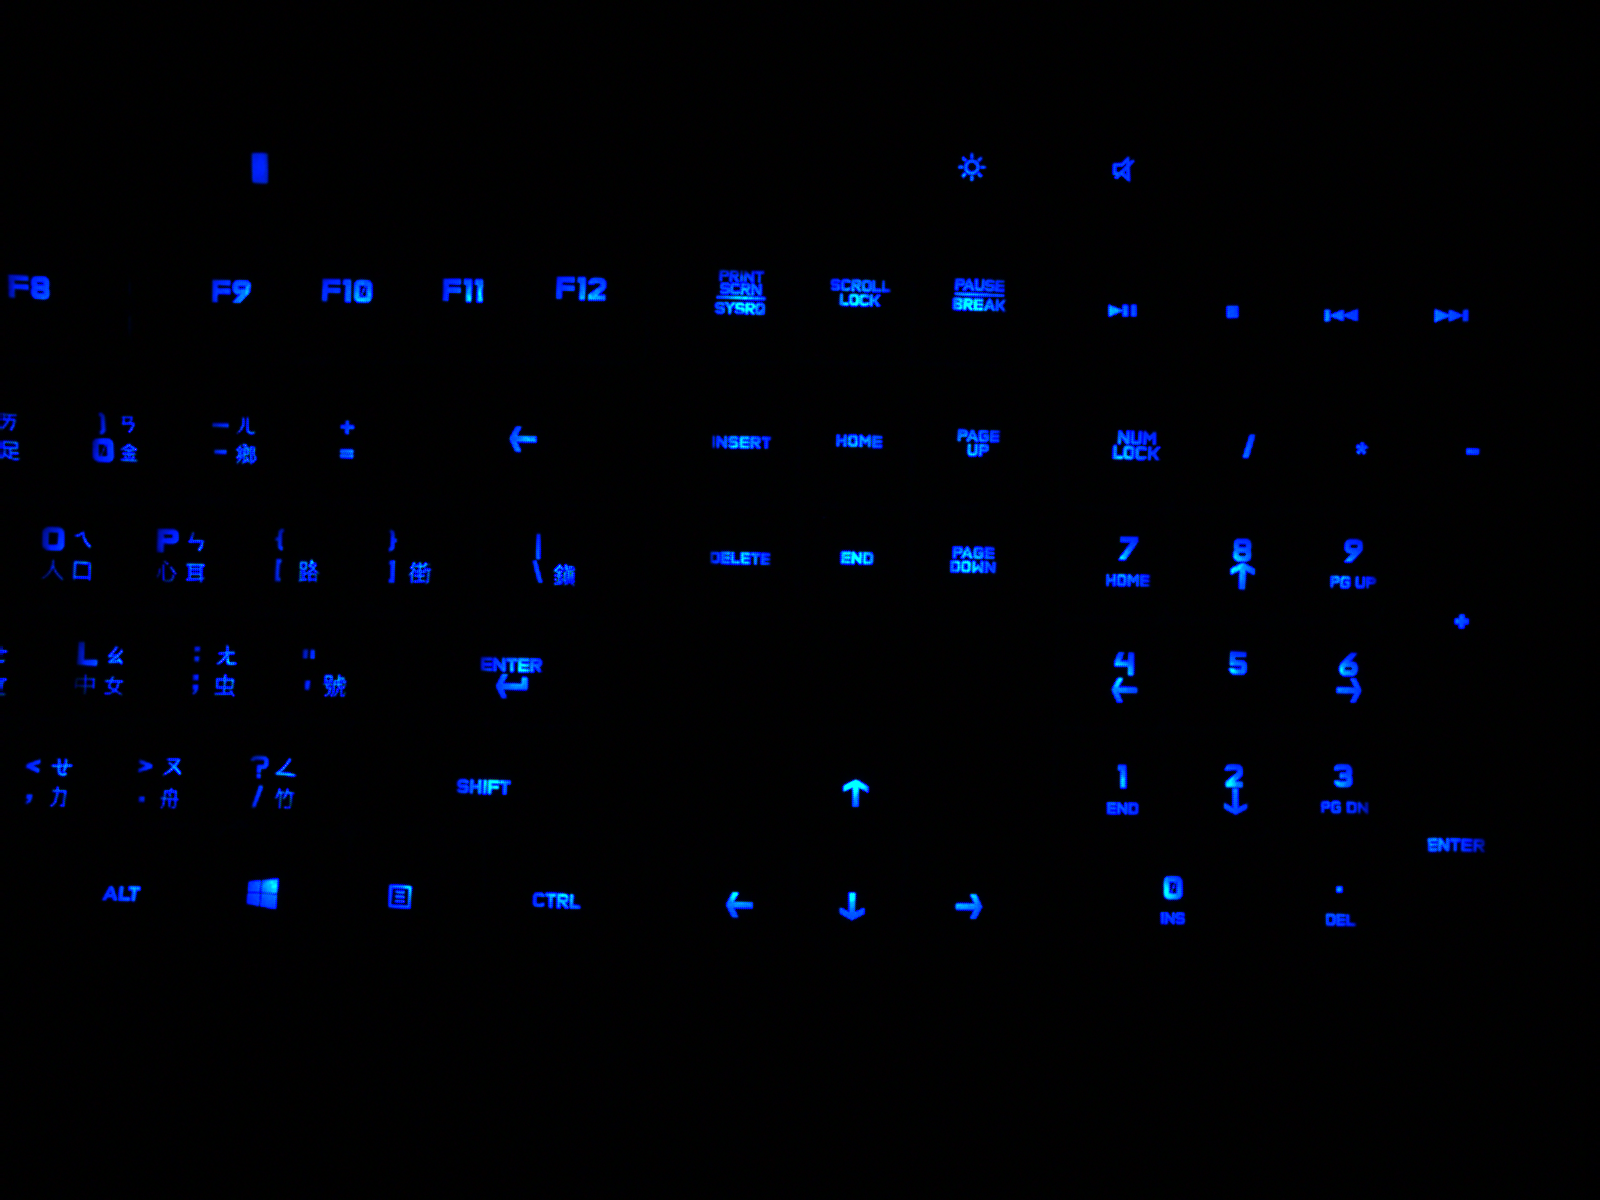
\includegraphics[width=0.5\linewidth]{simulation/normal/input_gold.png}
			}
			\subfigure[Sample Image without Adding Noises \& Distortion]
			{
				\includegraphics[width=0.5\linewidth]{simulation/normal/input_sample.png}
			}
			\caption{Input Images}
			\label{fig:RawImages}
		\end{figure}

		\subsubsection{SIFT}
		SIFT 
		\begin{figure}[H]
			\subfigure[Reference Image Feature Points]
			{
				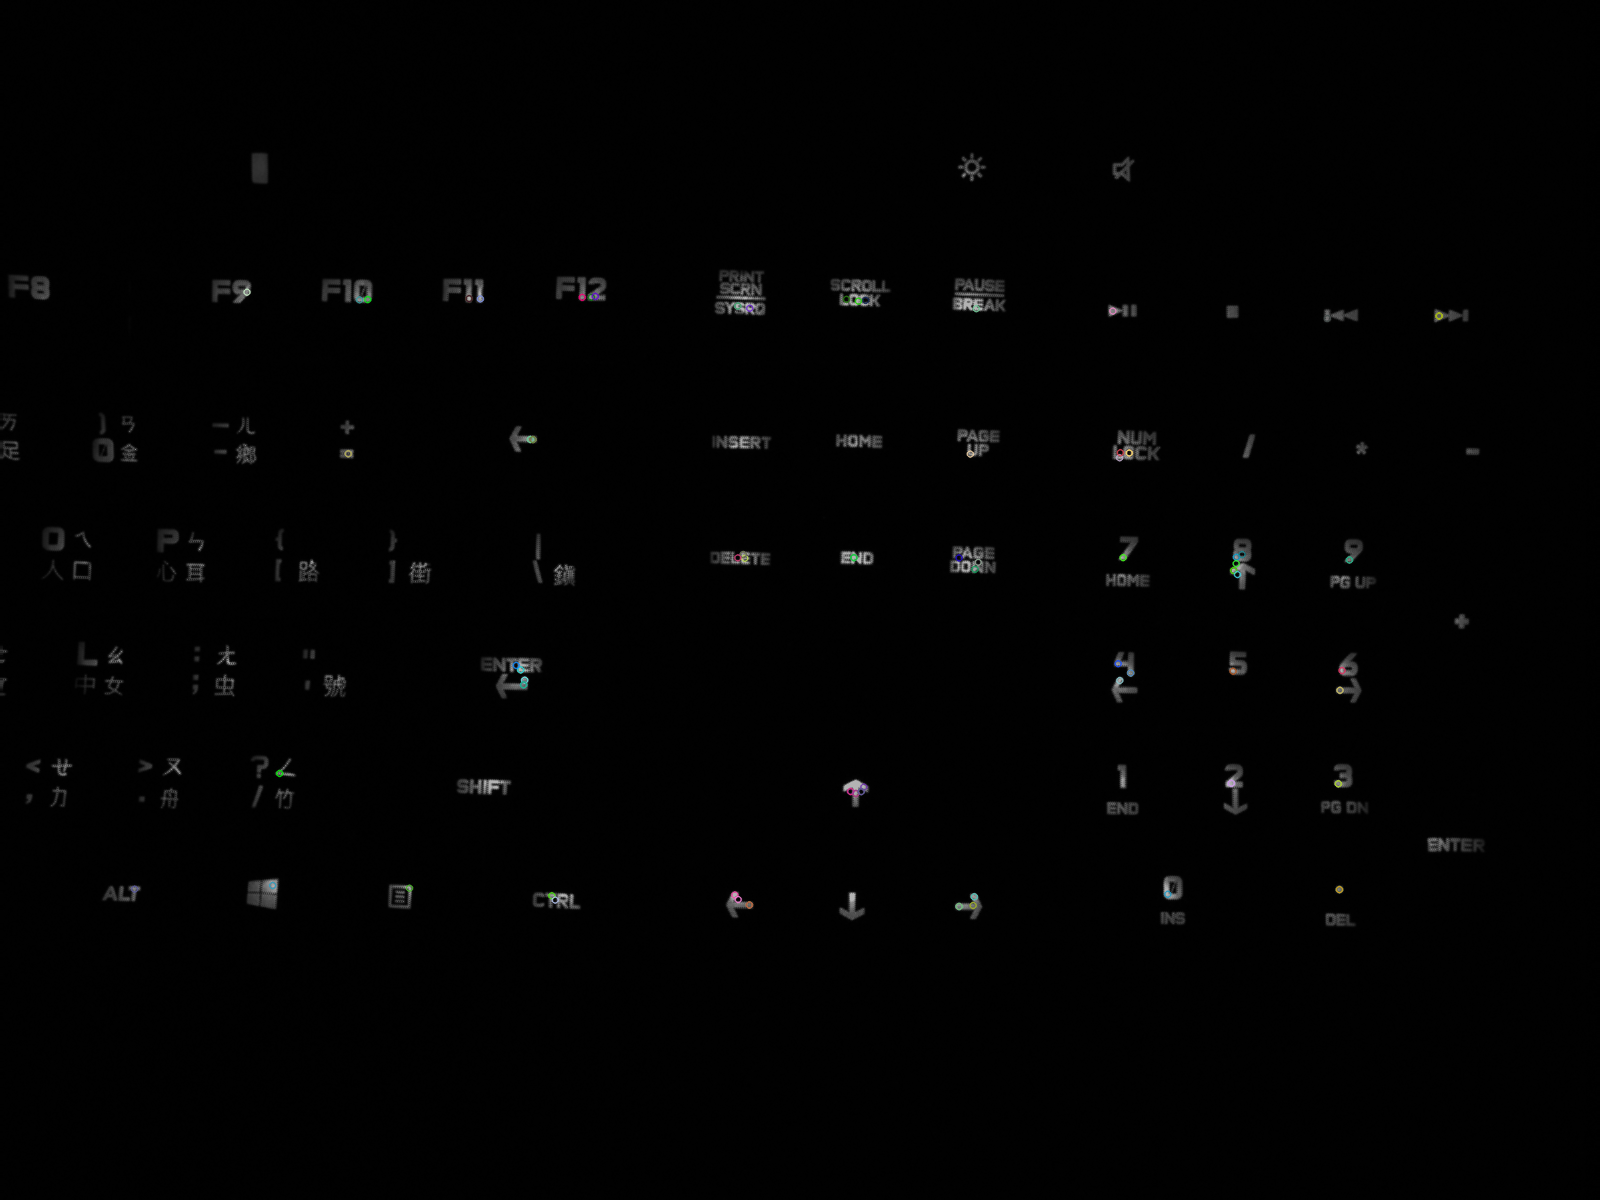
\includegraphics[width=0.5\linewidth]{simulation/normal/sift_gold_kp.png}
			}
			\subfigure[Sample Image Feature Points]
			{	
				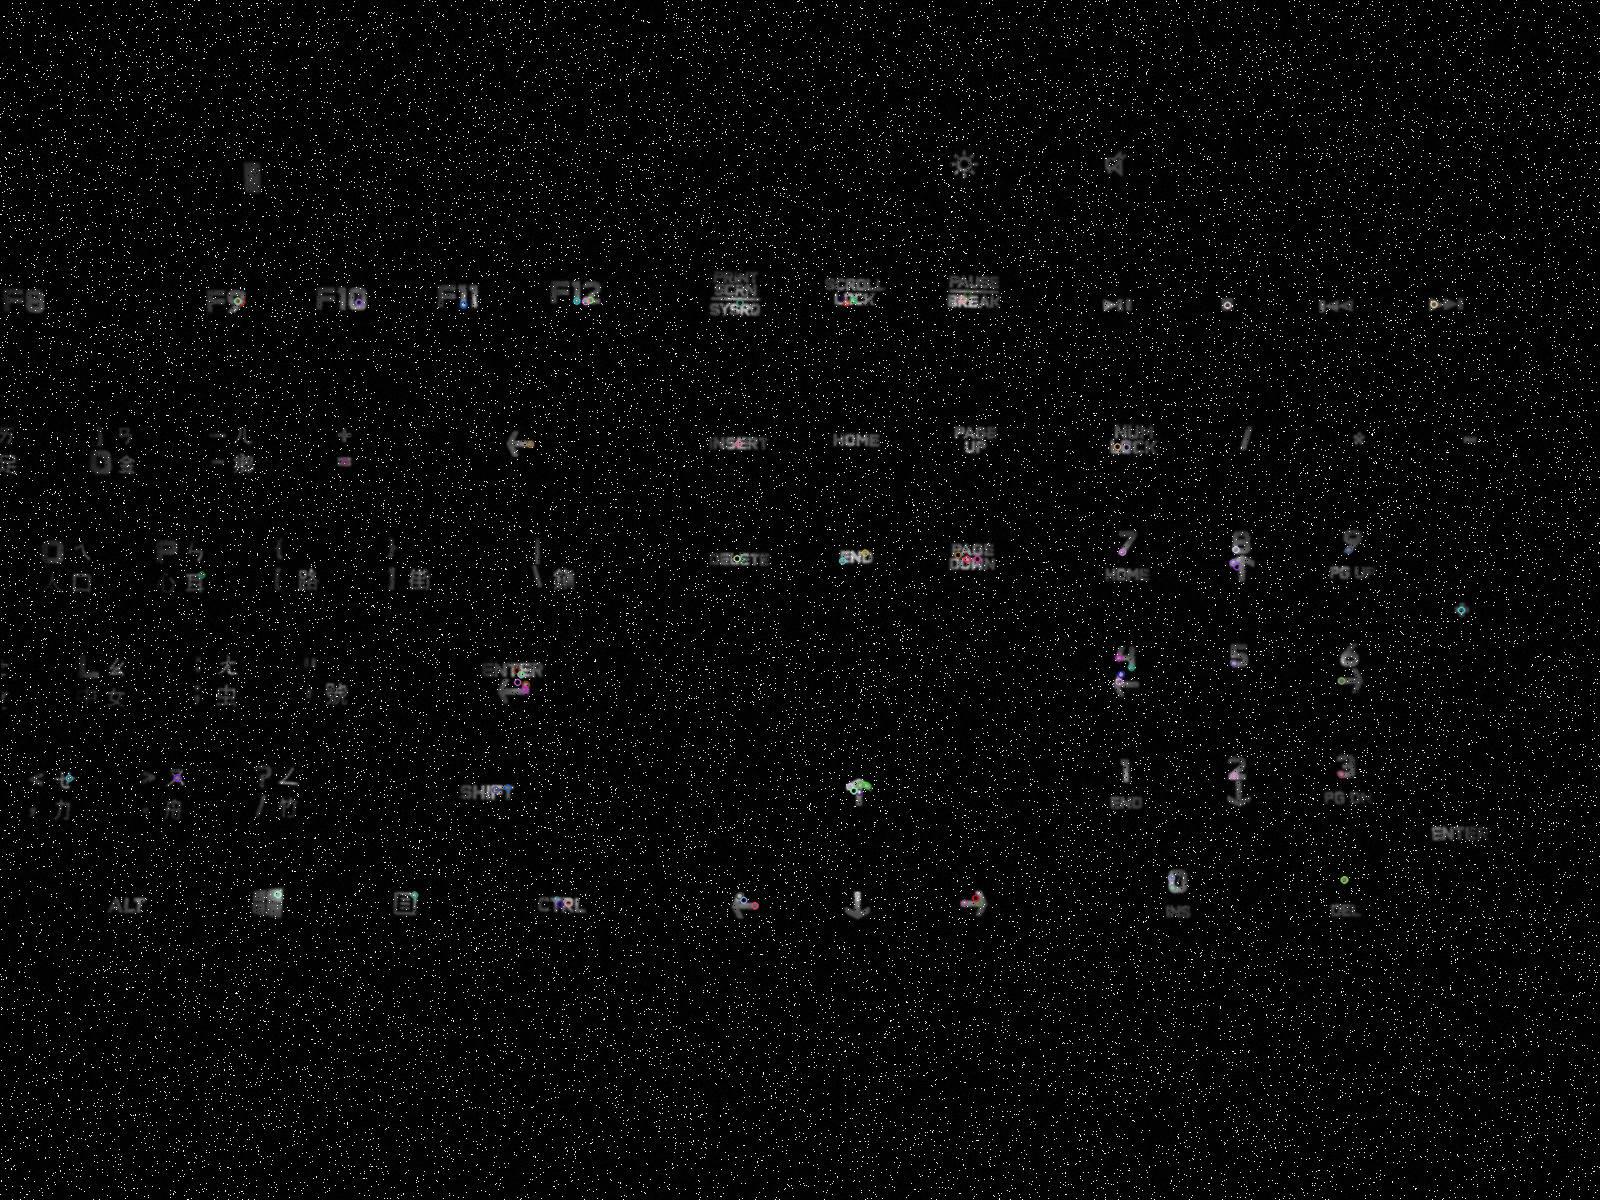
\includegraphics[width=0.5\linewidth]{simulation/normal/sift_sample_kp.png}
			}
			\caption{Reference and sample image after feature points were marked.}
			\label{fig:siftFeaturePoints}
		\end{figure}
		\begin{figure}[H]
			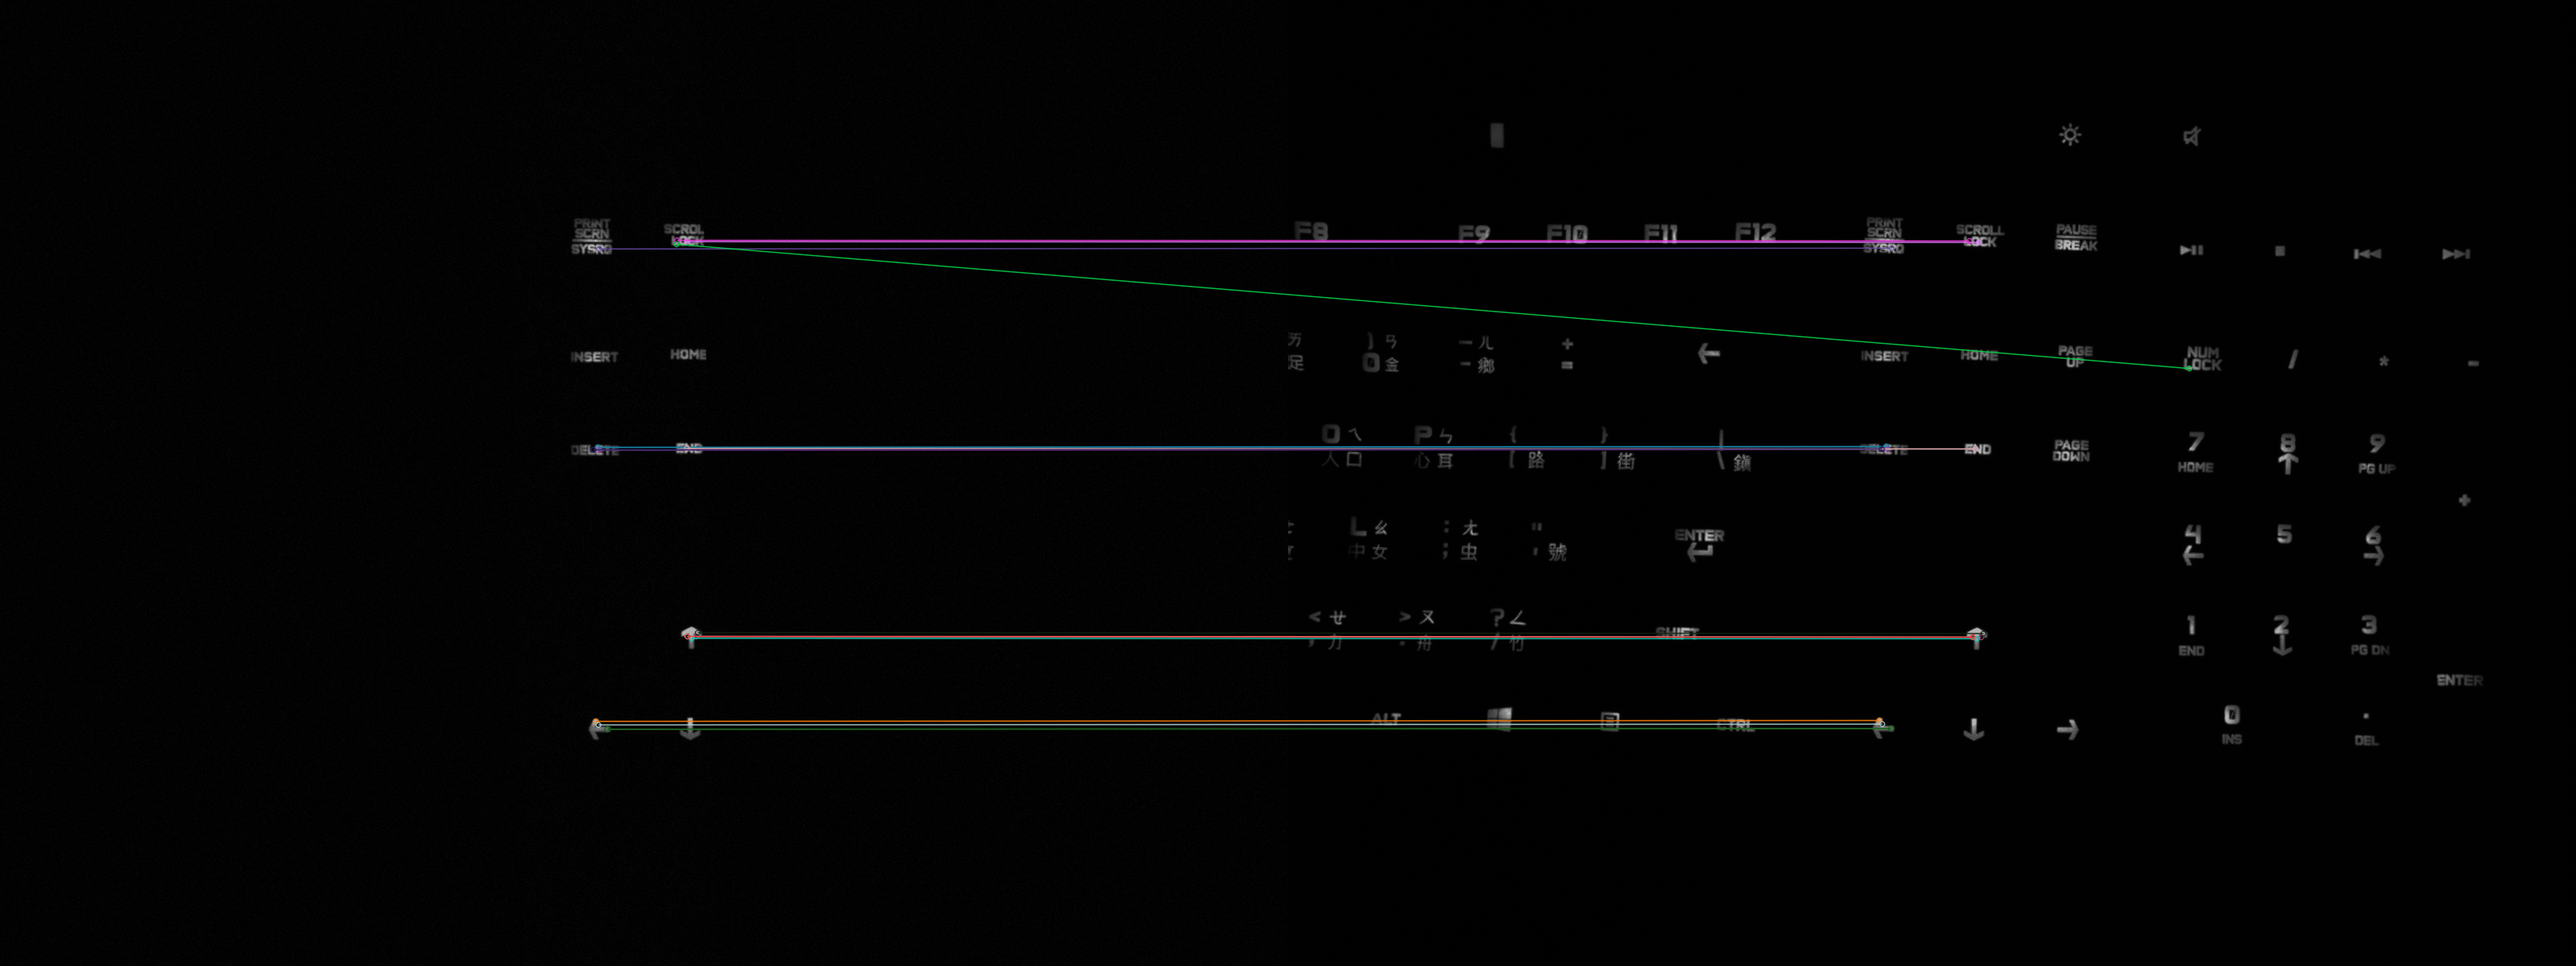
\includegraphics[width=\linewidth]{simulation/normal/sift_matches.png}
			\caption{Feature Point Matching Results}
			\label{fig:sifeMatchingResult}
		\end{figure}
		\begin{figure}[H]
			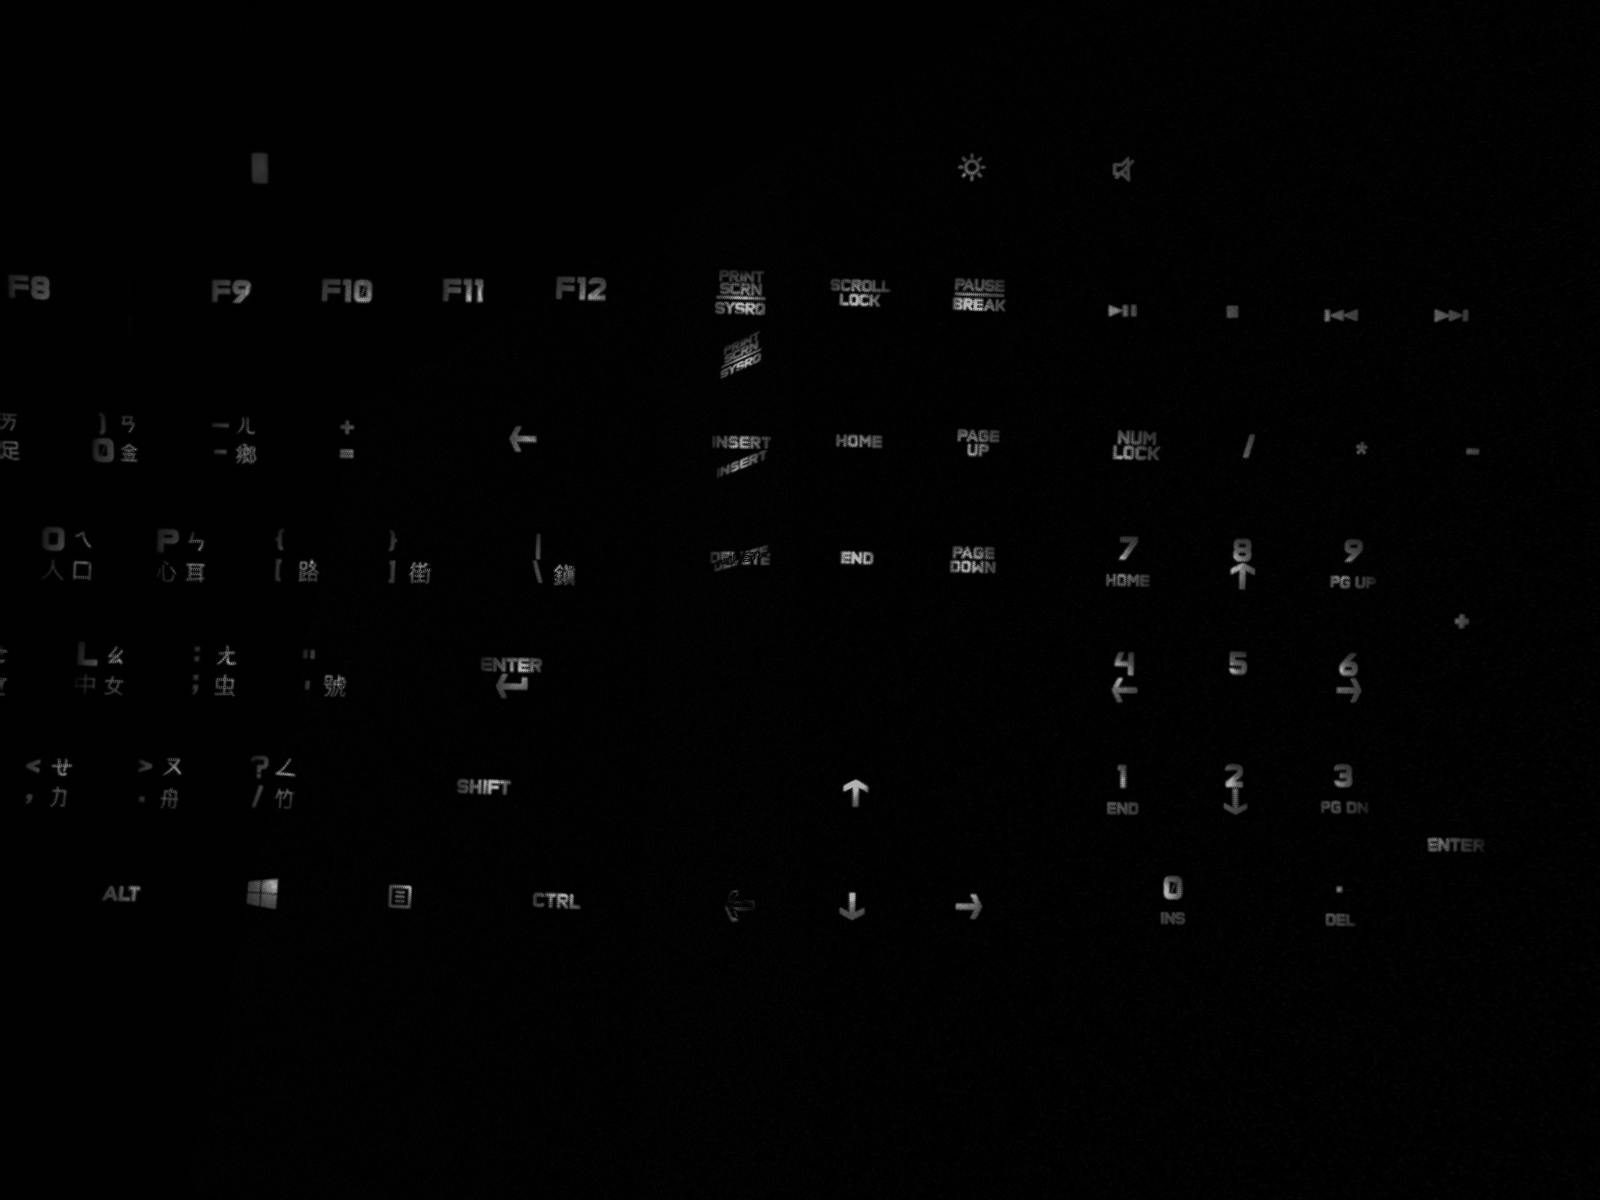
\includegraphics[width=\linewidth]{simulation/normal/sift_absdiff.png}
			\caption{Absolute Difference Results}
			\label{fig:siftAbsDifference}
		\end{figure}


		\subsubsection{SURF}
		\begin{figure}[H]
			\subfigure[Reference Image Feature Points]
			{
				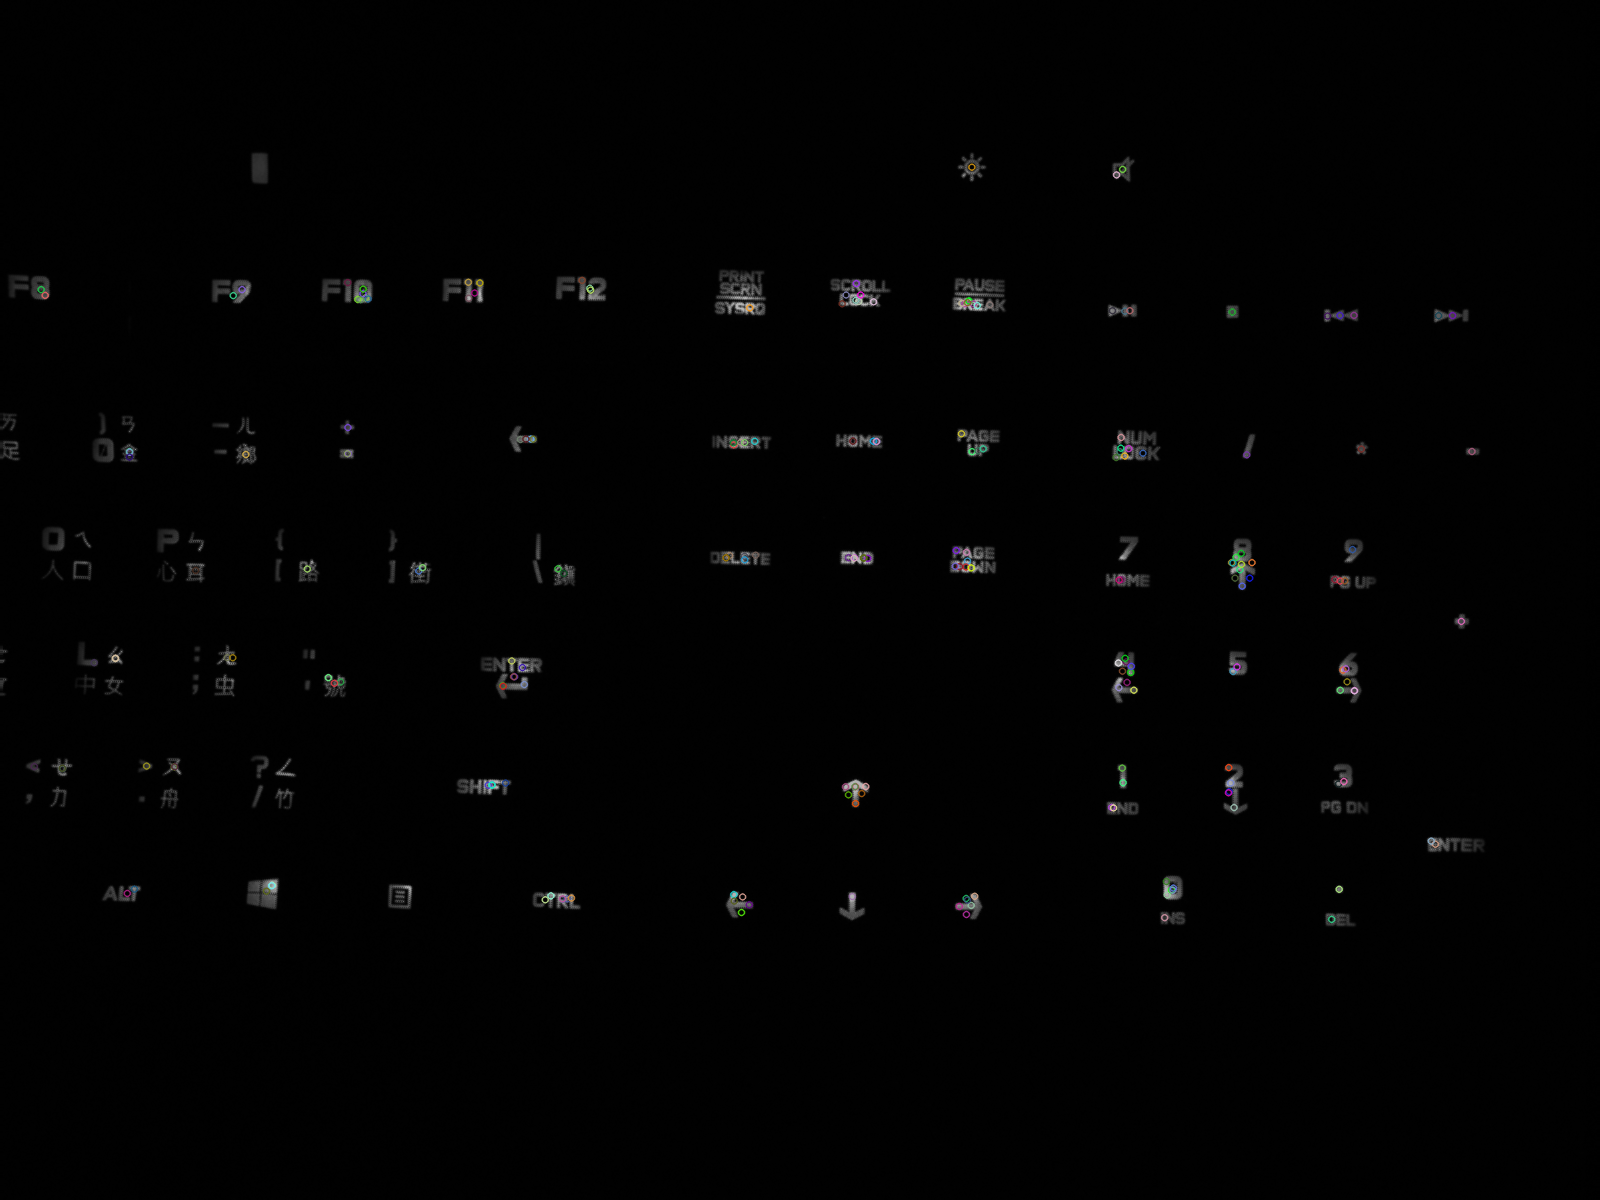
\includegraphics[width=0.5\linewidth]{simulation/normal/surf_gold_kp.png}
			}
			\subfigure[Sample Image Feature Points]
			{	
				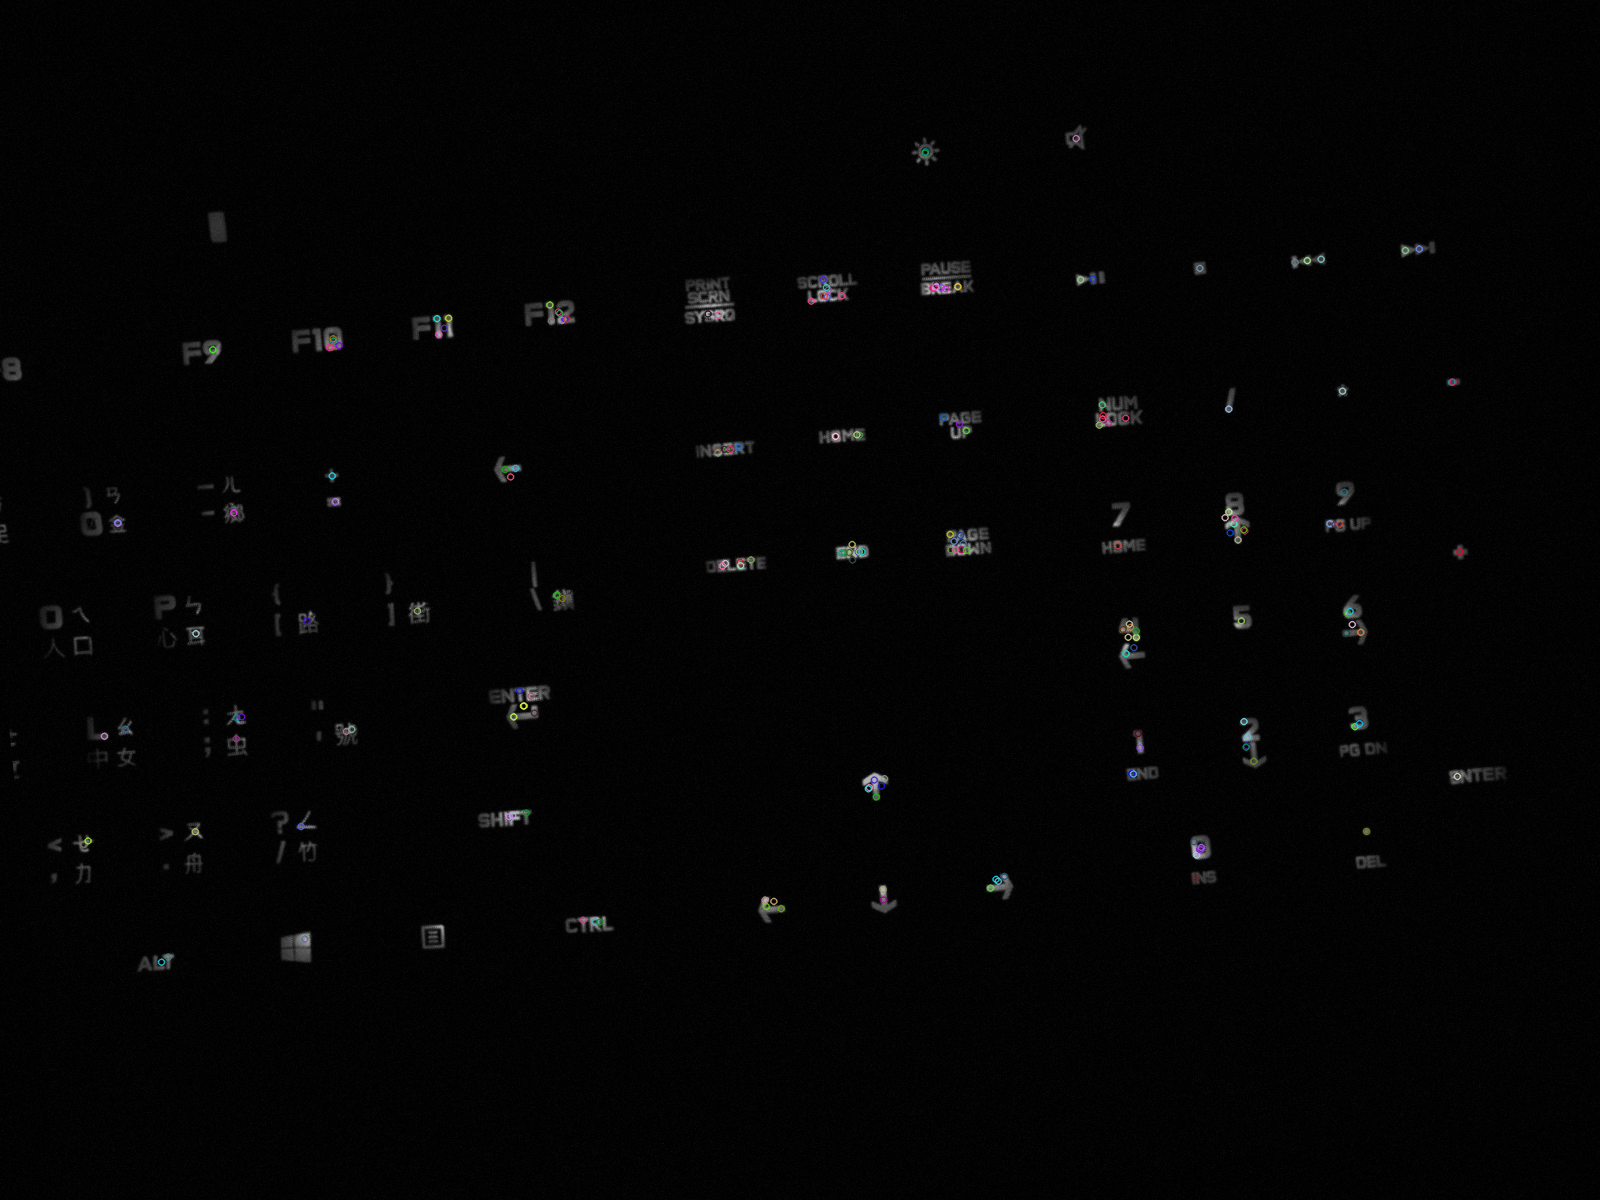
\includegraphics[width=0.5\linewidth]{simulation/normal/surf_sample_kp.png}
			}
			\caption{Reference and sample image after feature points were marked.}
			\label{fig:siftFeaturePoints}
		\end{figure}
		\begin{figure}[H]
			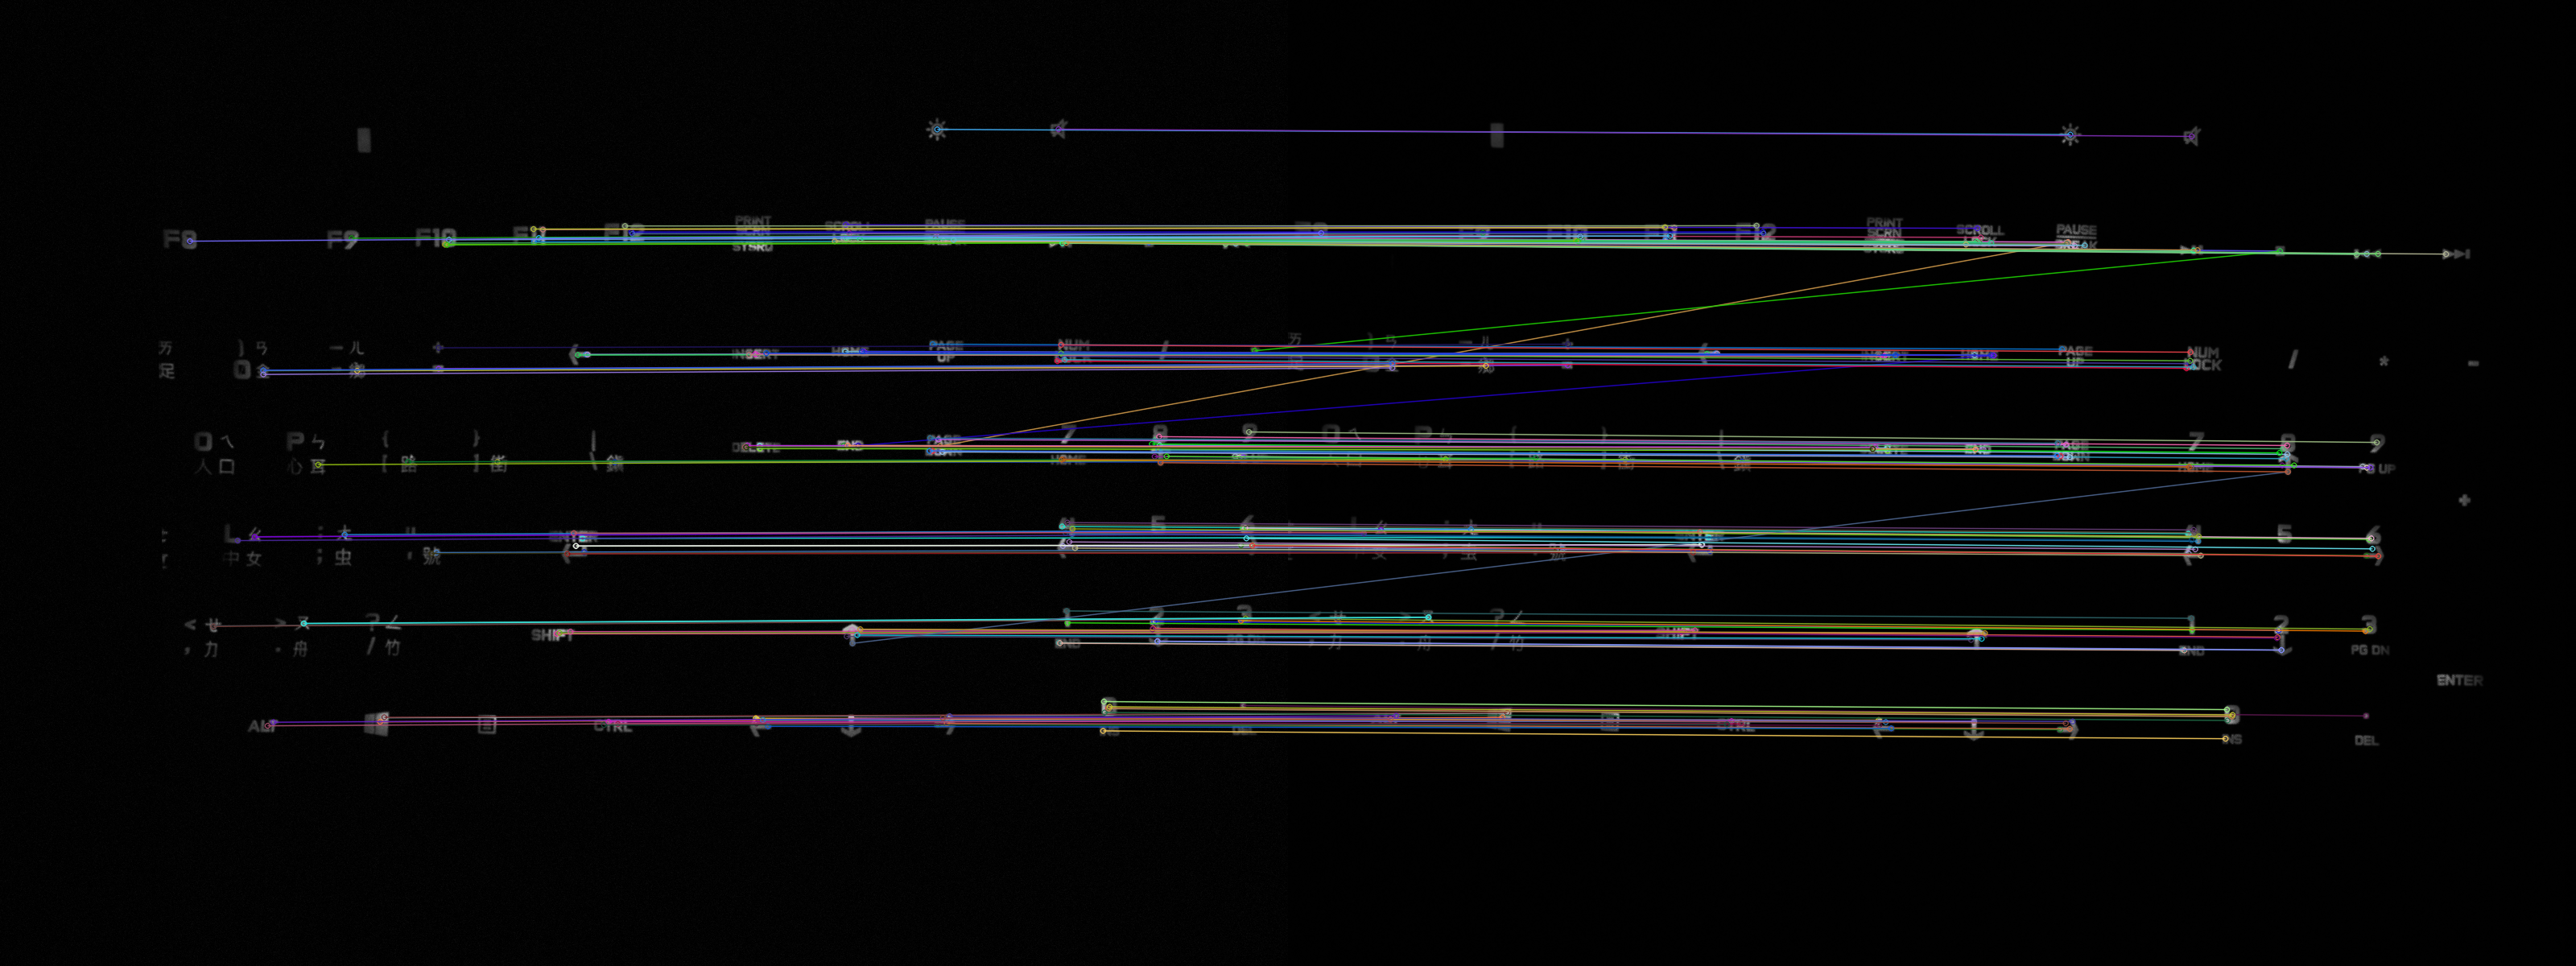
\includegraphics[width=\linewidth]{simulation/normal/surf_matches.png}
			\caption{Feature Point Matching Results}
			\label{fig:sifeMatchingResult}
		\end{figure}
		\begin{figure}[H]
			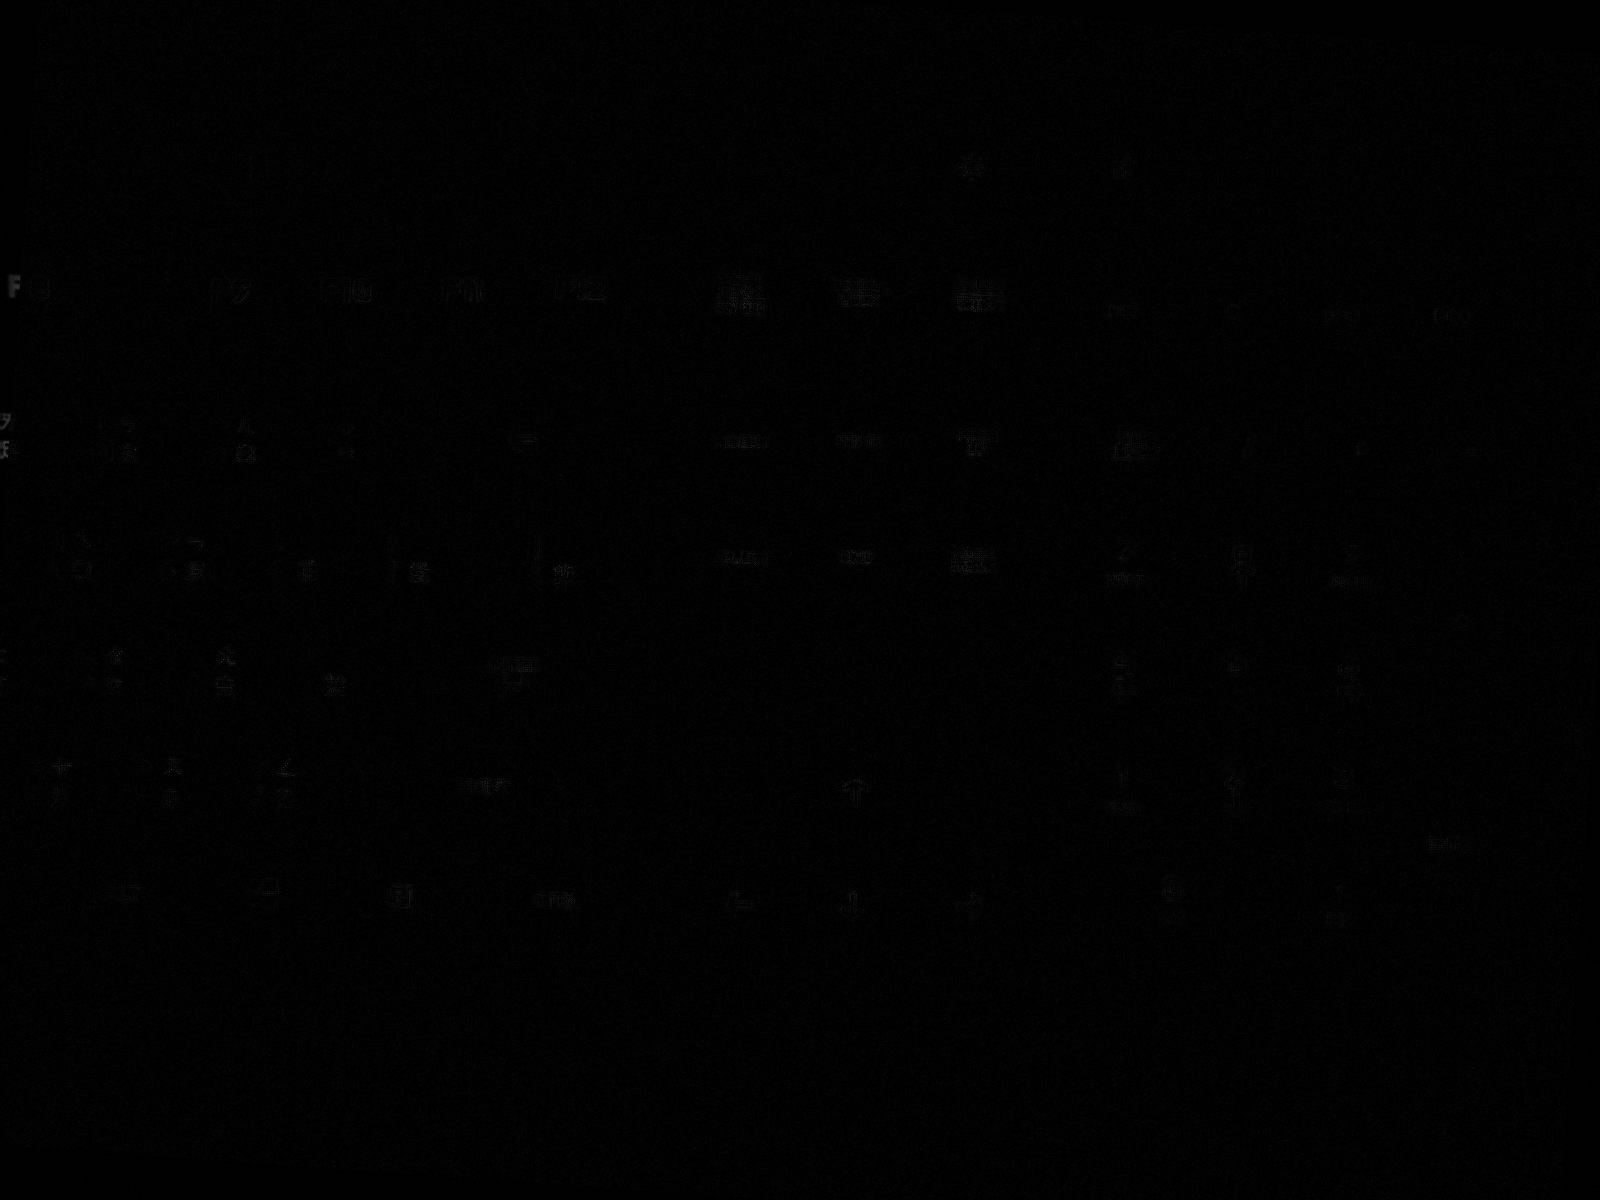
\includegraphics[width=\linewidth]{simulation/normal/surf_absdiff.png}
			\caption{Absolute Difference Results}
			\label{fig:siftAbsDifference}
		\end{figure}


		\subsubsection{ORB}
		\begin{figure}[H]
			\subfigure[Reference Image Feature Points]
			{
				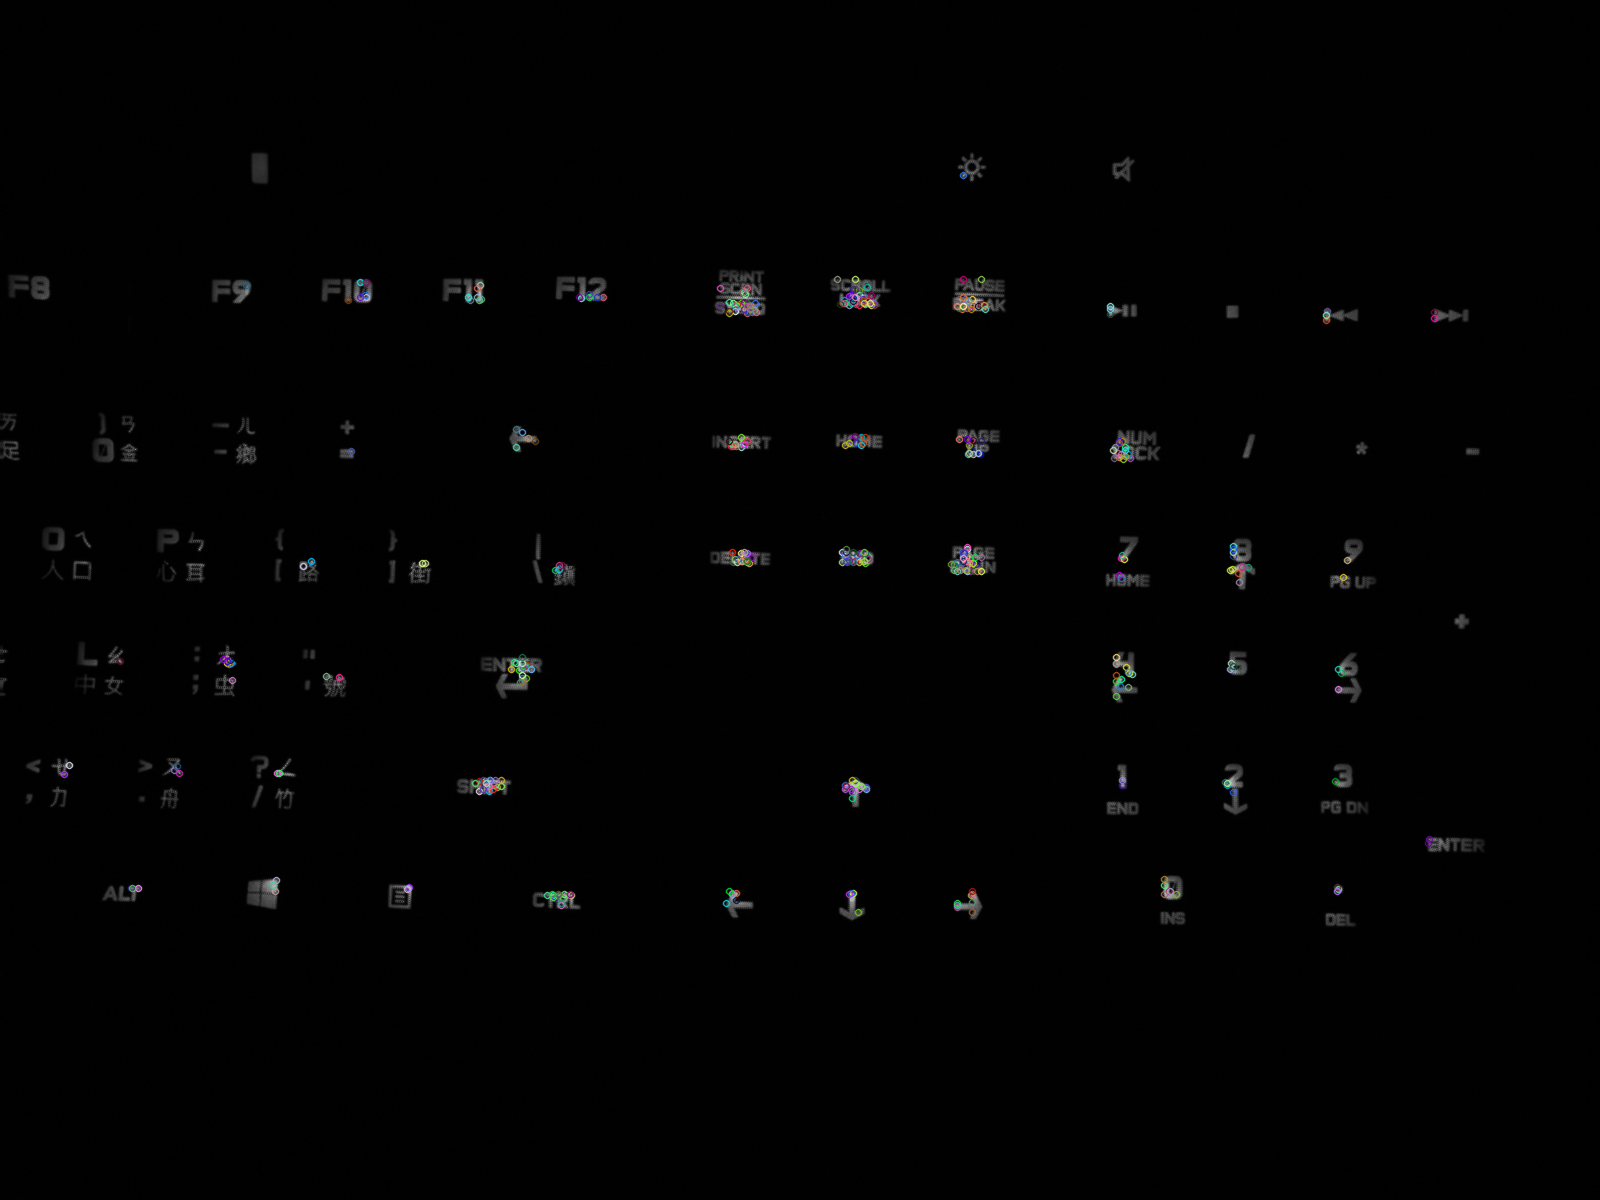
\includegraphics[width=0.5\linewidth]{simulation/normal/orb_gold_kp.png}
			}
			\subfigure[Sample Image Feature Points]
			{	
				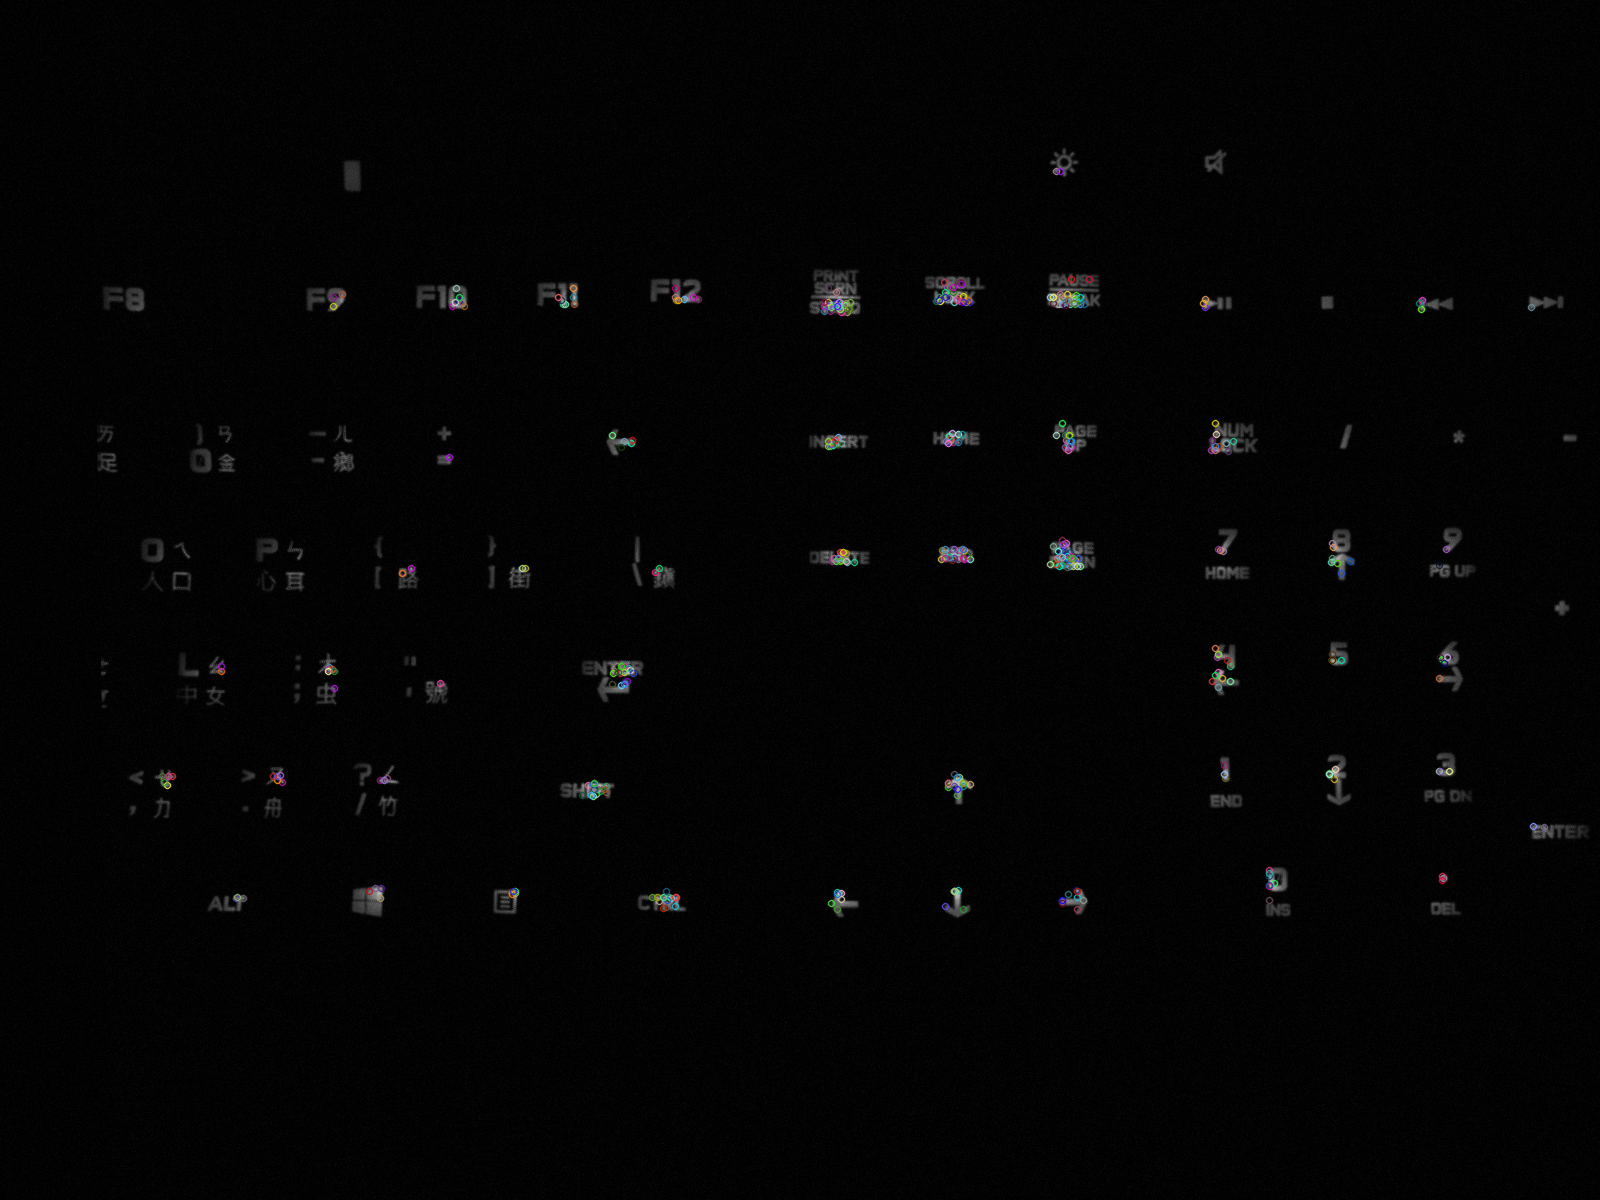
\includegraphics[width=0.5\linewidth]{simulation/normal/orb_sample_kp.png}
			}
			\caption{Reference and sample image after feature points were marked.}
			\label{fig:siftFeaturePoints}
		\end{figure}
		\begin{figure}[H]
			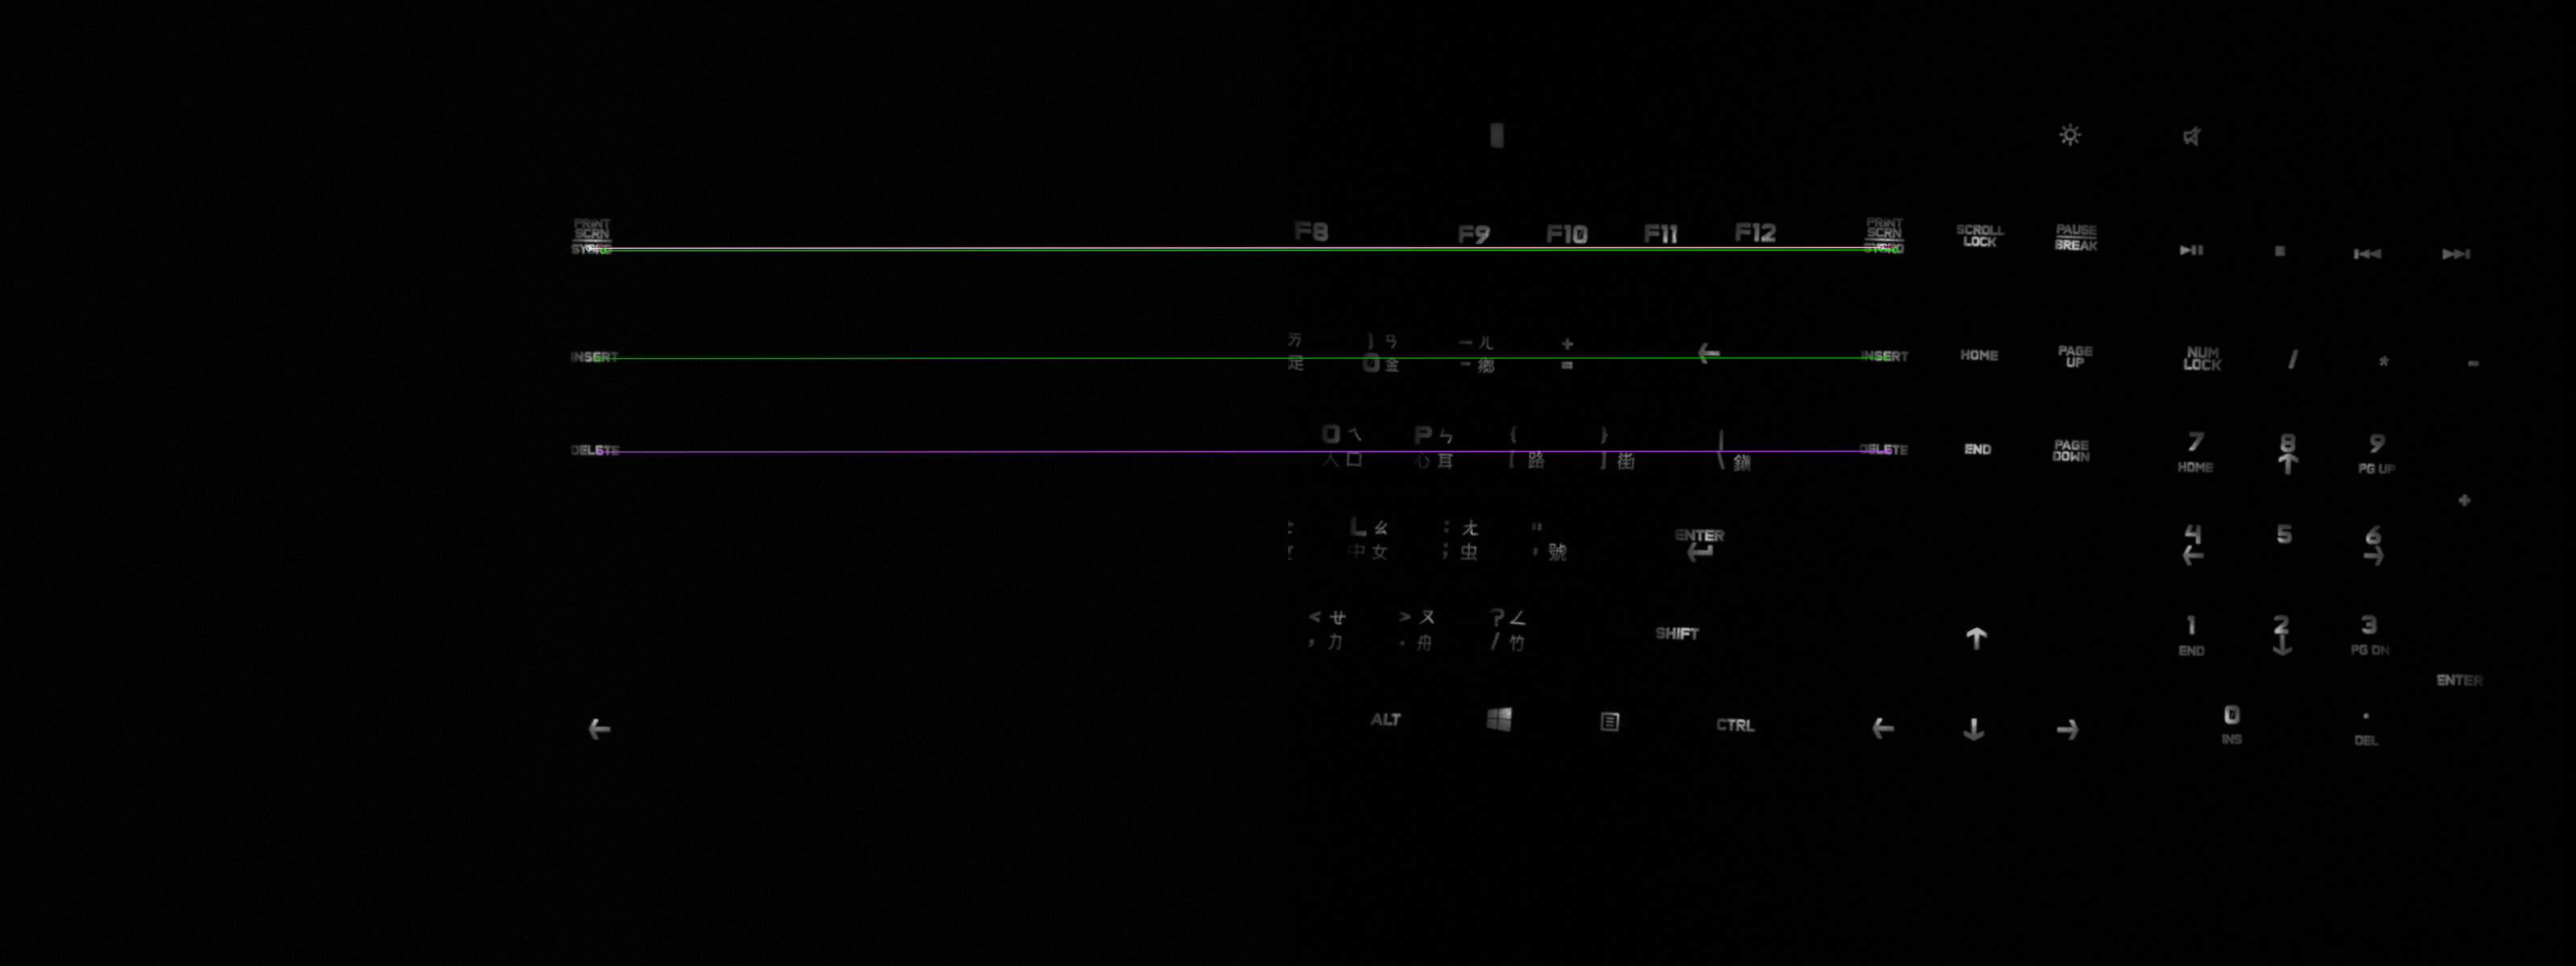
\includegraphics[width=\linewidth]{simulation/normal/orb_matches.png}
			\caption{Feature Point Matching Results}
			\label{fig:sifeMatchingResult}
		\end{figure}
		\begin{figure}[H]
			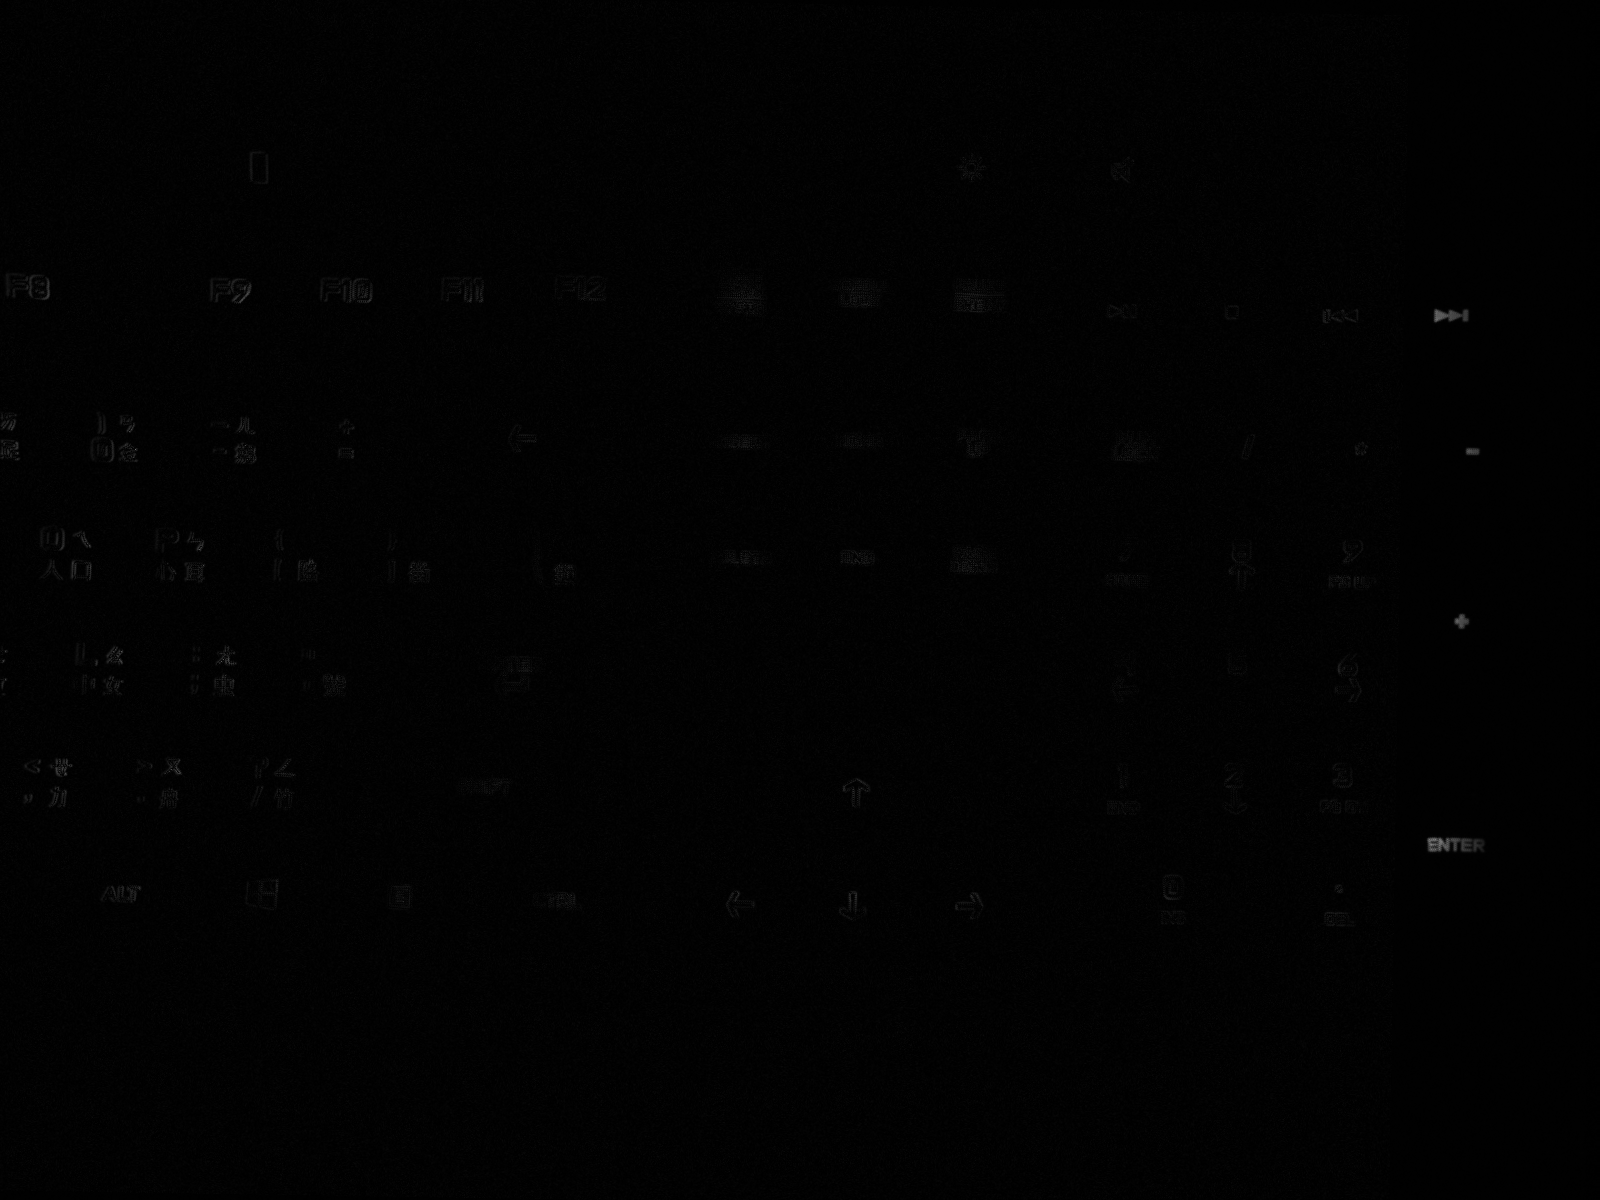
\includegraphics[width=\linewidth]{simulation/normal/orb_absdiff.png}
			\caption{Absolute Difference Results}
			\label{fig:siftAbsDifference}
		\end{figure}

		\subsubsection{AKAZE}
		\begin{figure}[H]
			\subfigure[Reference Image Feature Points]
			{
				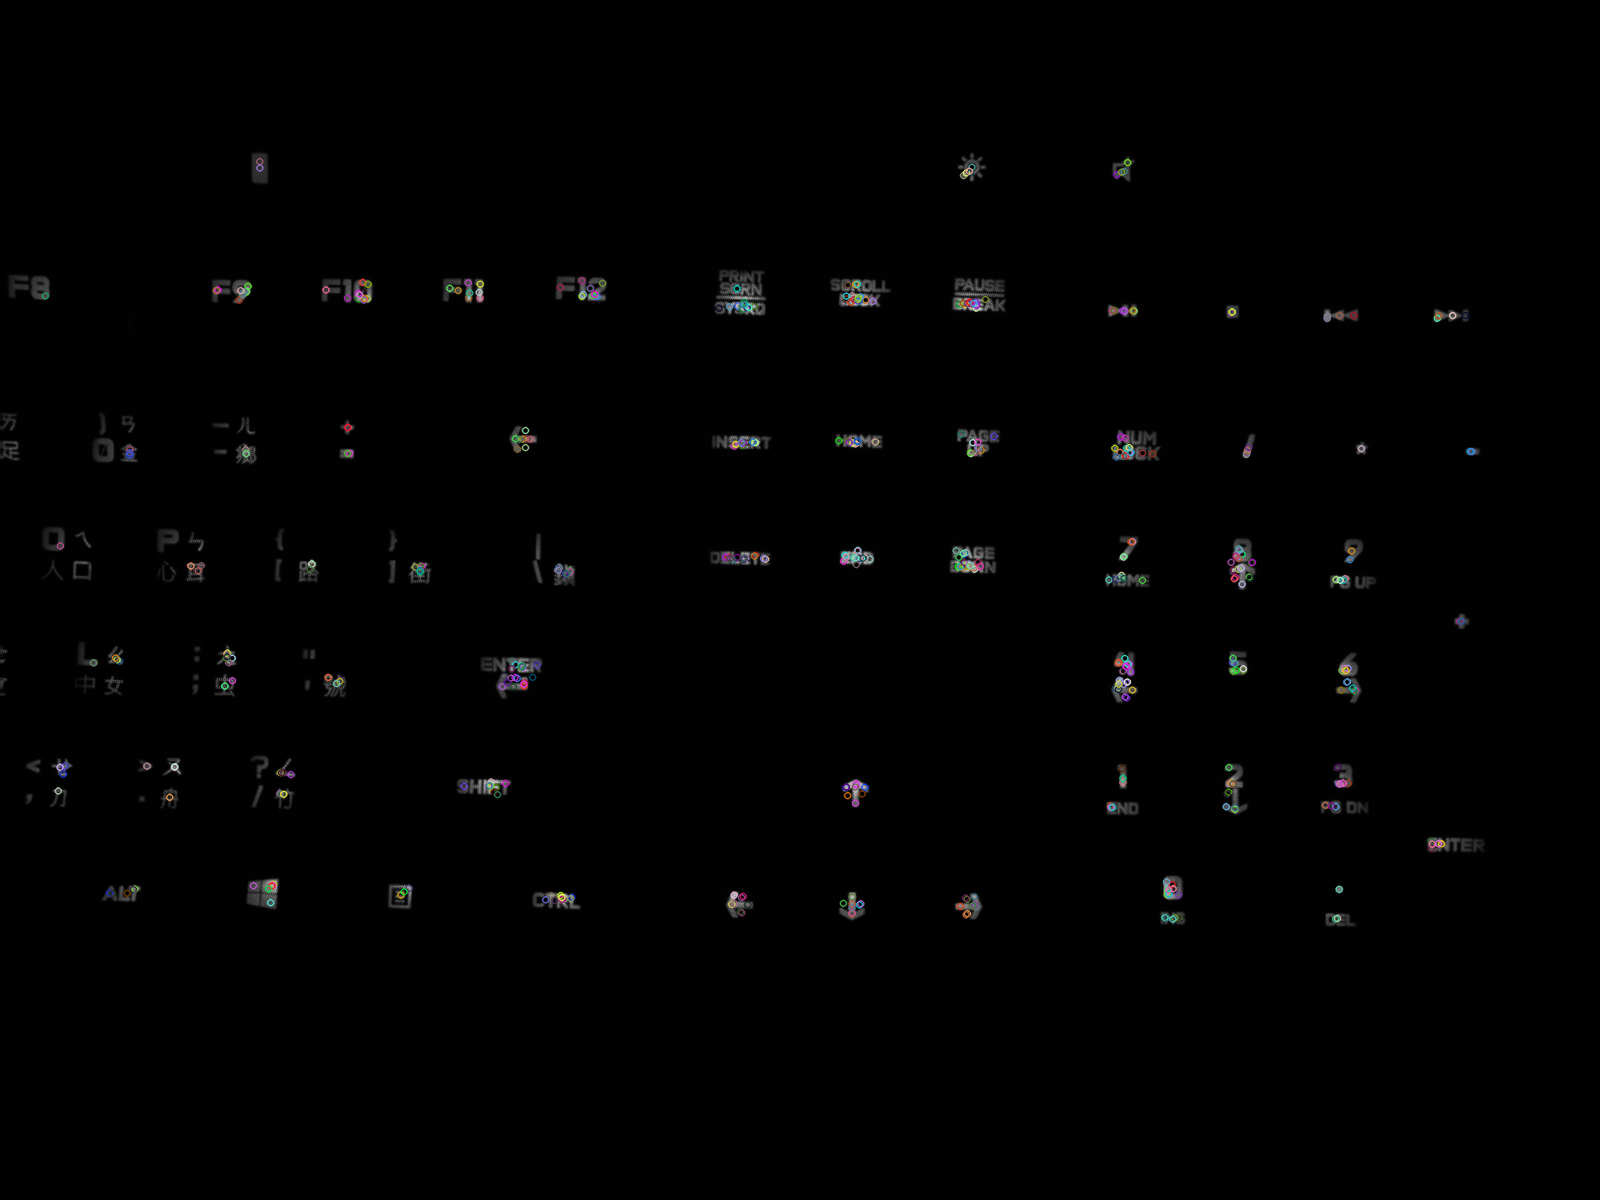
\includegraphics[width=0.5\linewidth]{simulation/normal/akaze_gold_kp.png}
			}
			\subfigure[Sample Image Feature Points]
			{	
				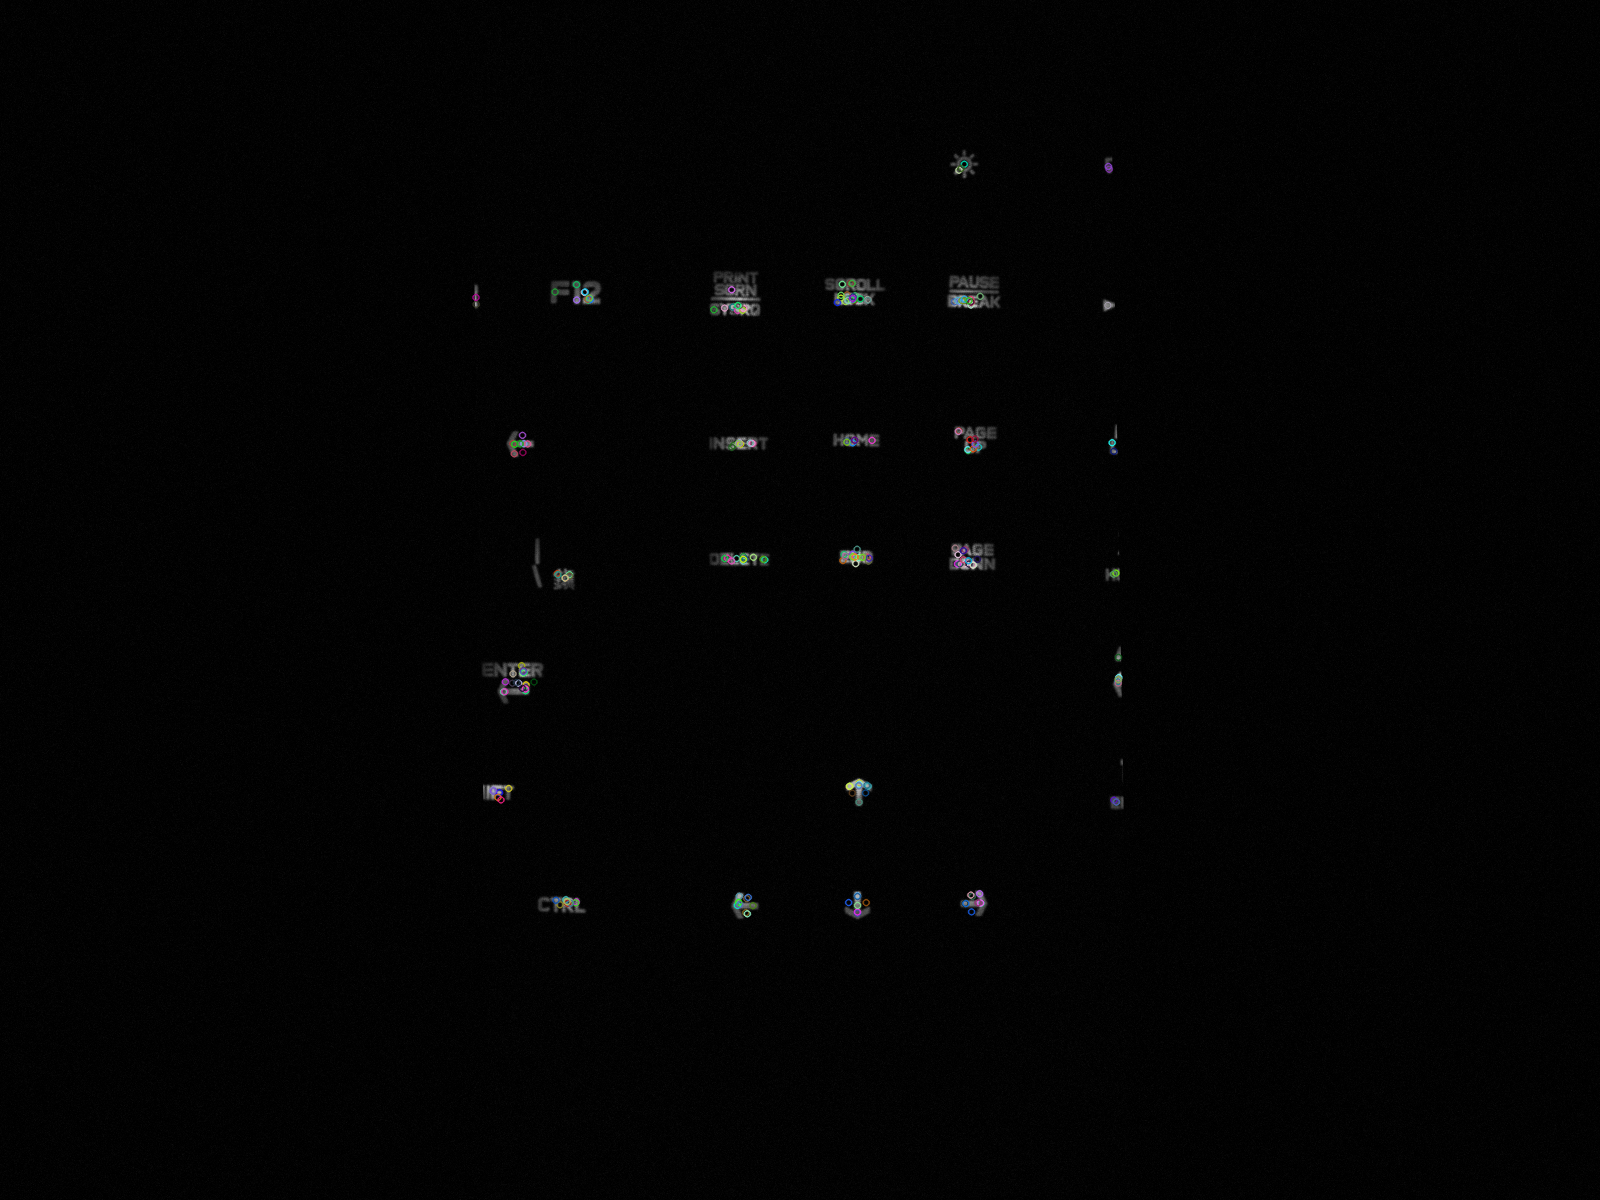
\includegraphics[width=0.5\linewidth]{simulation/normal/akaze_sample_kp.png}
			}
			\caption{Reference and sample image after feature points were marked.}
			\label{fig:siftFeaturePoints}
		\end{figure}
		\begin{figure}[H]
			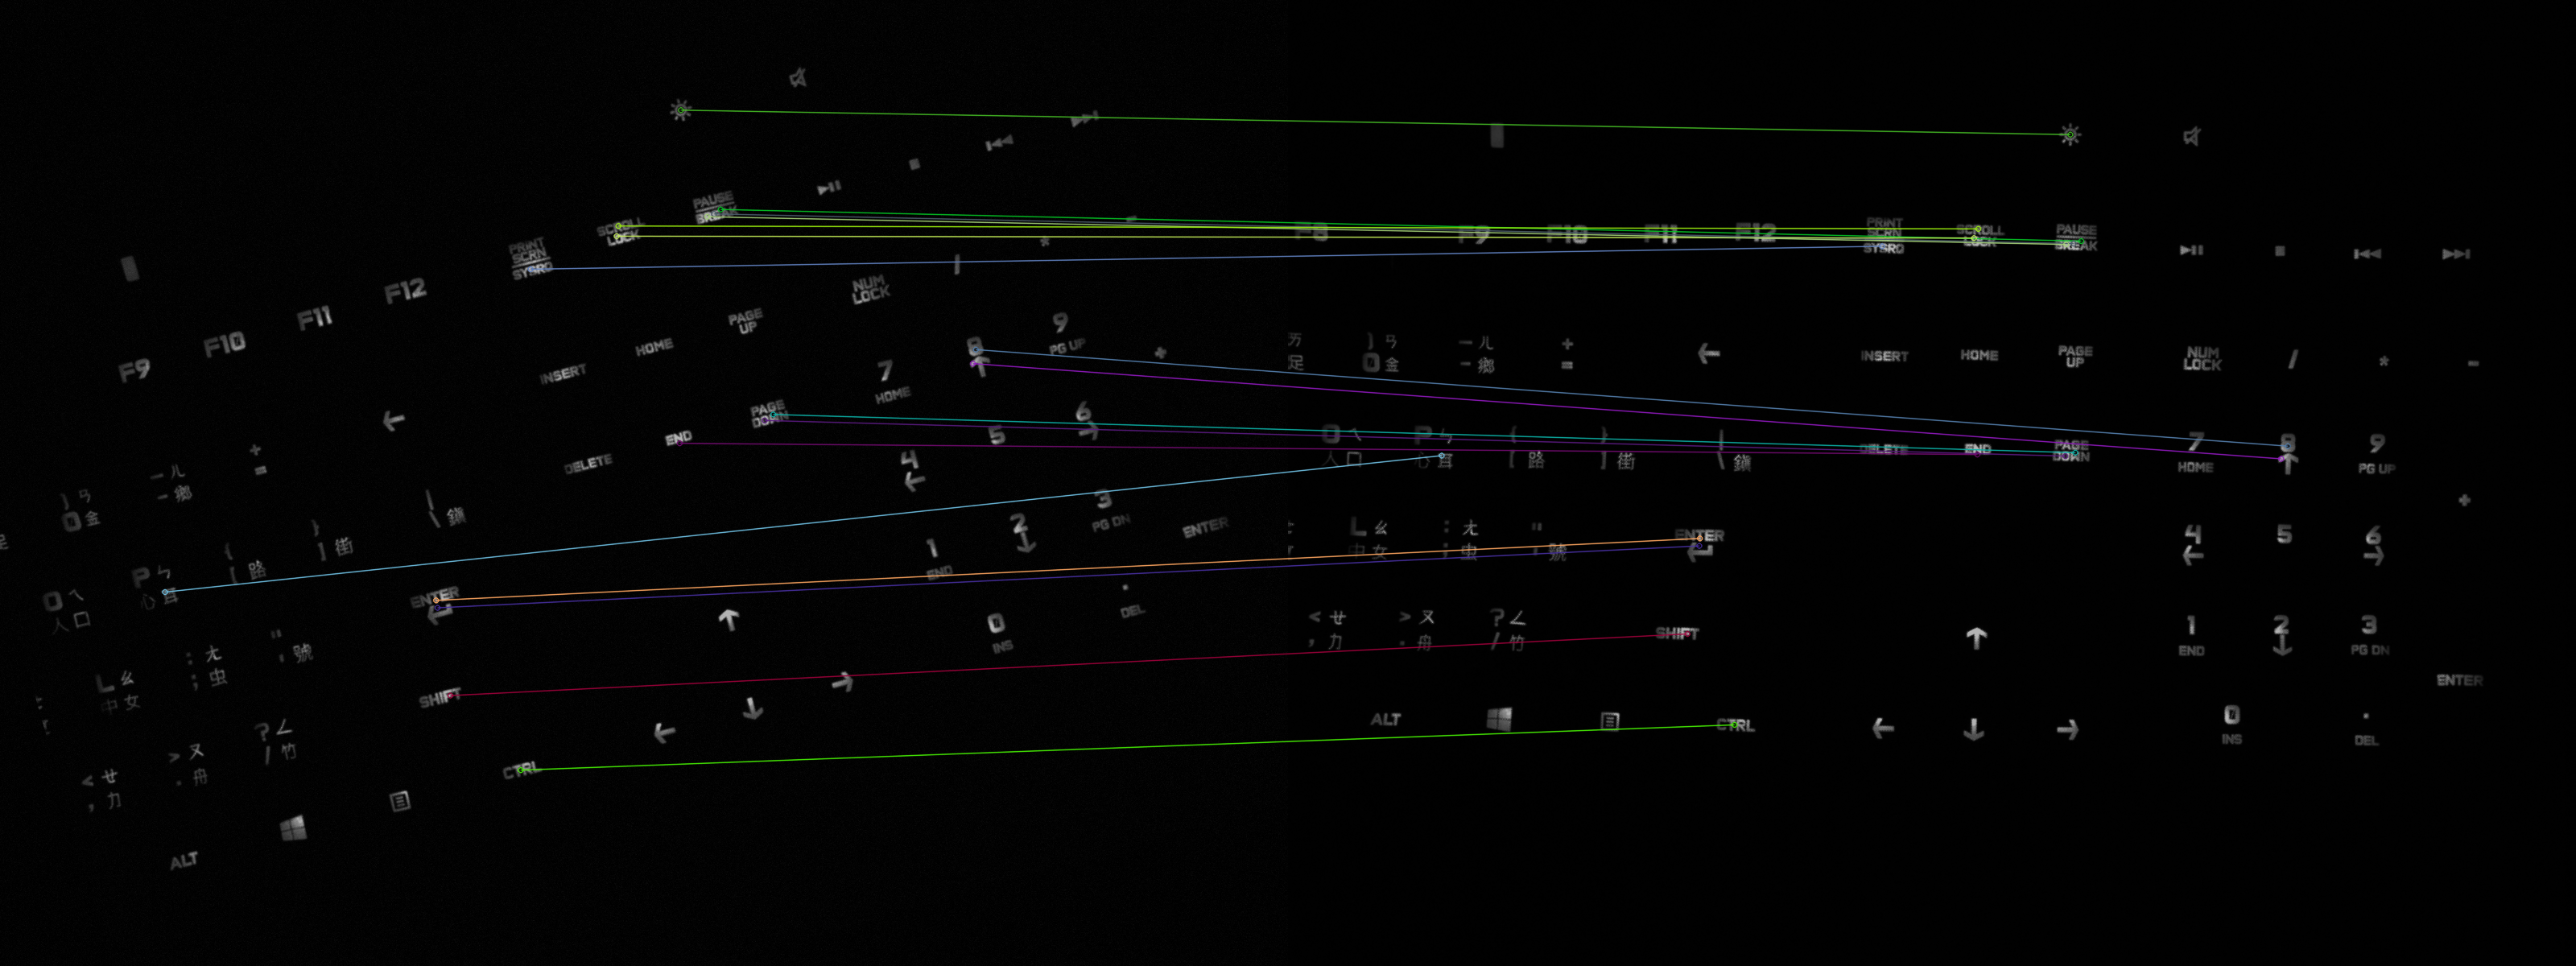
\includegraphics[width=\linewidth]{simulation/normal/akaze_matches.png}
			\caption{Feature Point Matching Results}
			\label{fig:sifeMatchingResult}
		\end{figure}
		\begin{figure}[H]
			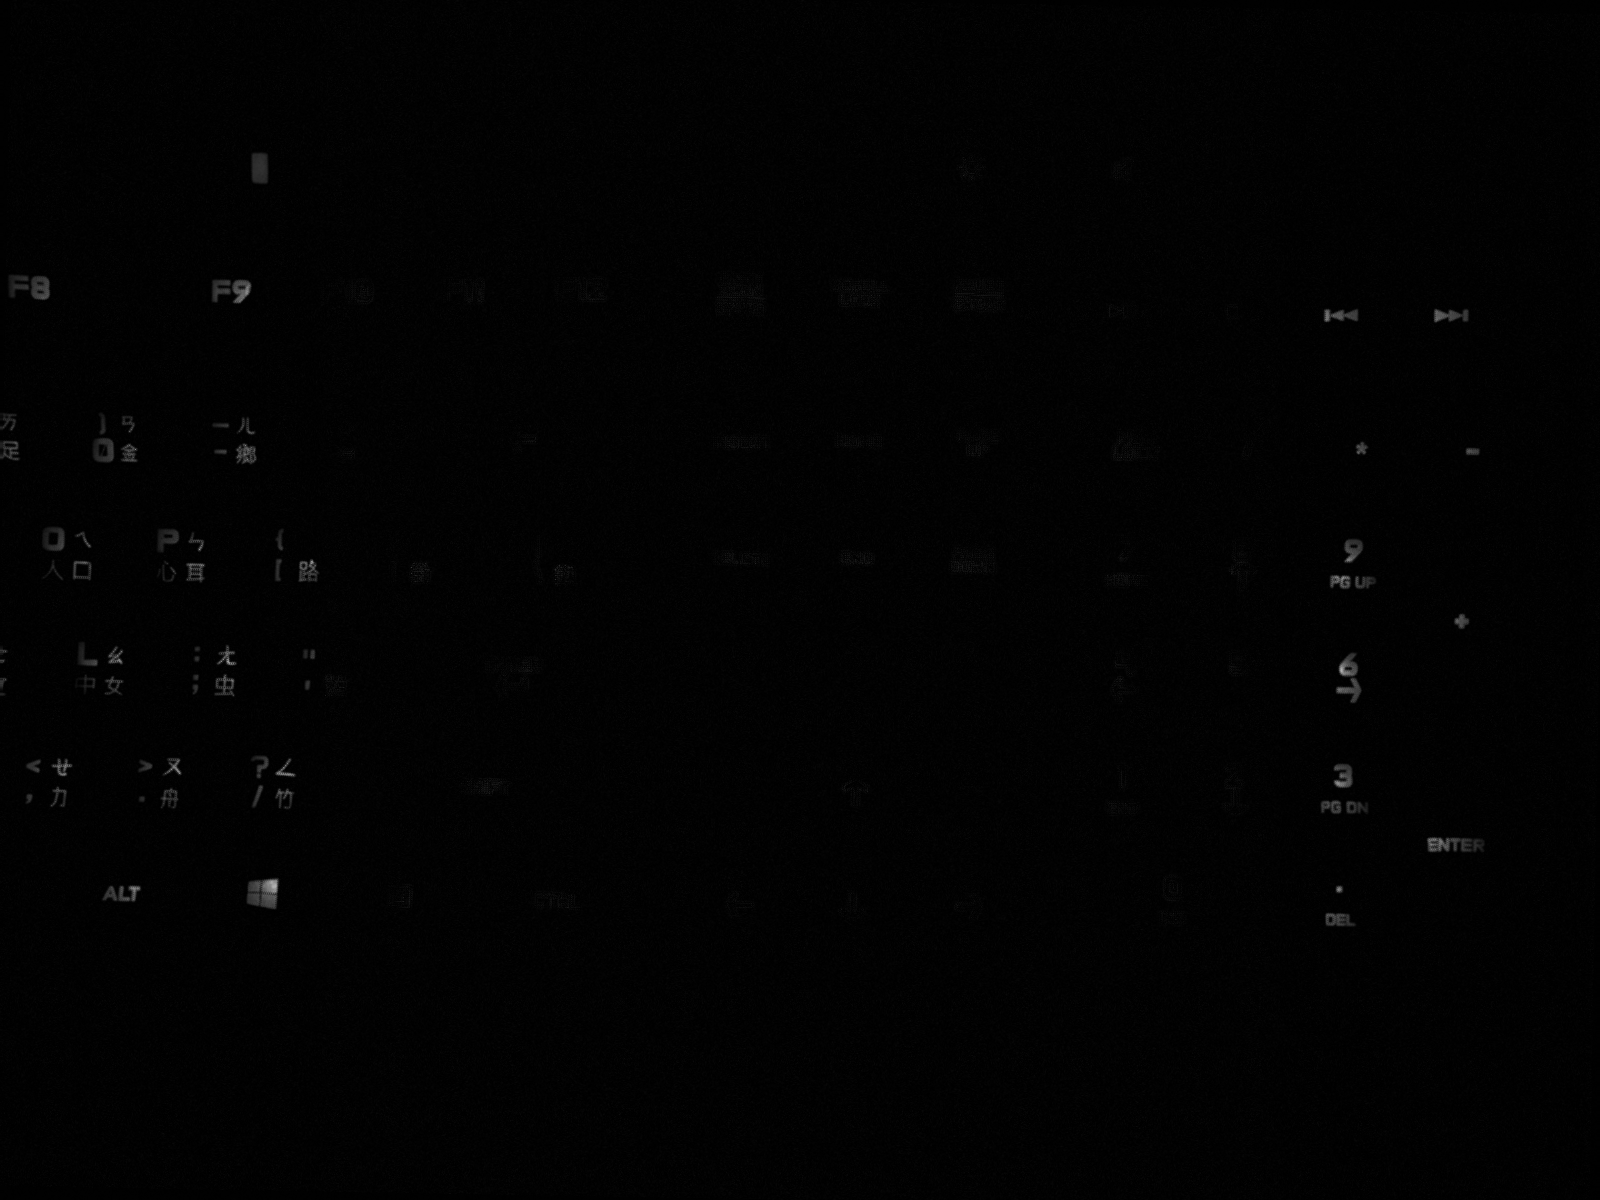
\includegraphics[width=\linewidth]{simulation/normal/akaze_absdiff.png}
			\caption{Absolute Difference Results}
			\label{fig:siftAbsDifference}
		\end{figure}
	\subsection{Unexpected Rotate}
		In this section, we'll rotate the sample image \ref{fig:testSamplesOfRotation} from 1 to 10 degree and 15 degree and 20 degree then observe the difference between each feature detector. 
		In this case, ORB feature detector starts have chance to have a bad alignment when rotation is over 3 degrees, while others still could have good alignment result under 15 degrees of rotation. 
		When the rotation increased over 15 degree, SURF detector start to have bad alignment since we set the SURF detector to be the Upright-SURF in the implementation, this makes the SURF detector having better time efficiency but lower performance under unexpected rotation.
		In the production line, the fixture we used to doing this examination would only allow a rotation under 1 degree happening.
		\begin{figure}[H]
			\subfigure[Reference Image]
			{
				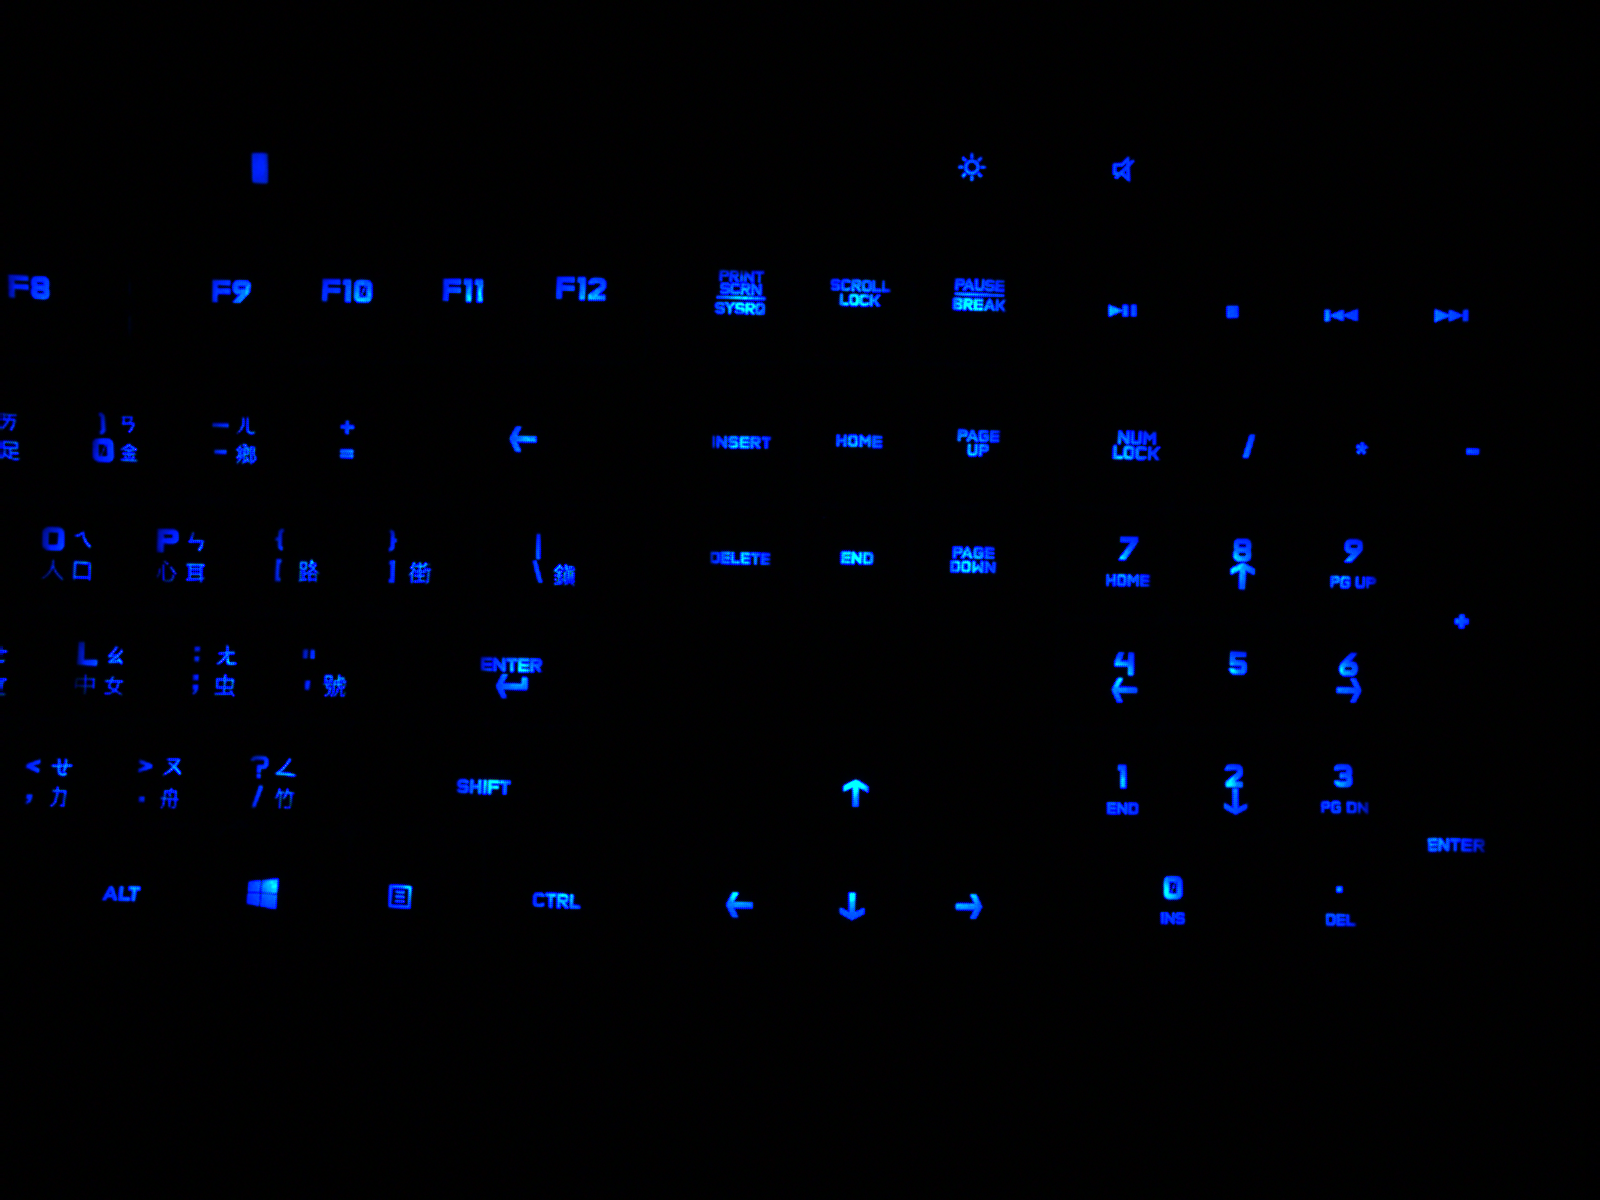
\includegraphics[width=0.3\linewidth]{simulation/normal/input_gold.png}
			}
			\subfigure[1 Degree Rotation]
			{
				\includegraphics[width=0.3\linewidth]{simulation/Rotation/1/input_sample.png}
			}
			\subfigure[2 Degree Rotation]
			{
				\includegraphics[width=0.3\linewidth]{simulation/Rotation/2/input_sample.png}
			}
			\subfigure[3 Degree Rotation]
			{
				\includegraphics[width=0.3\linewidth]{simulation/Rotation/3/input_sample.png}
			}
			\subfigure[4 Degree Rotation]
			{
				\includegraphics[width=0.3\linewidth]{simulation/Rotation/4/input_sample.png}
			}
			\subfigure[5 Degree Rotation]
			{
				\includegraphics[width=0.3\linewidth]{simulation/Rotation/5/input_sample.png}
			}
			\subfigure[6 Degree Rotation]
			{
				\includegraphics[width=0.3\linewidth]{simulation/Rotation/6/input_sample.png}
			}
			\subfigure[7 Degree Rotation]
			{
				\includegraphics[width=0.3\linewidth]{simulation/Rotation/7/input_sample.png}
			}
			\subfigure[8 Degree Rotation]
			{
				\includegraphics[width=0.3\linewidth]{simulation/Rotation/8/input_sample.png}
			}
			\subfigure[9 Degree Rotation]
			{
				\includegraphics[width=0.3\linewidth]{simulation/Rotation/9/input_sample.png}
			}
			\subfigure[10 Degree Rotation]
			{
				\includegraphics[width=0.3\linewidth]{simulation/Rotation/10/input_sample.png}
			}
			\subfigure[15 Degree Rotation]
			{
				\includegraphics[width=0.3\linewidth]{simulation/Rotation/15/input_sample.png}
			}
			\subfigure[20 Degree Rotation]
			{
				\includegraphics[width=0.3\linewidth]{simulation/Rotation/20/input_sample.png}
			}
			\caption{Rotated Sample Image}
			\label{fig:testSamplesOfRotation}
		\end{figure}

		\begin{figure}[H]
			\subfigure[ORB Feature Detectors Result in 3 Degrees Rotation]
			{
				\includegraphics[width=0.5\linewidth]{simulation/Rotation/3/orb_showDefect.png}
			}
			\subfigure[SURF Feature Detectors Result in 3 Degrees Rotation]
			{
				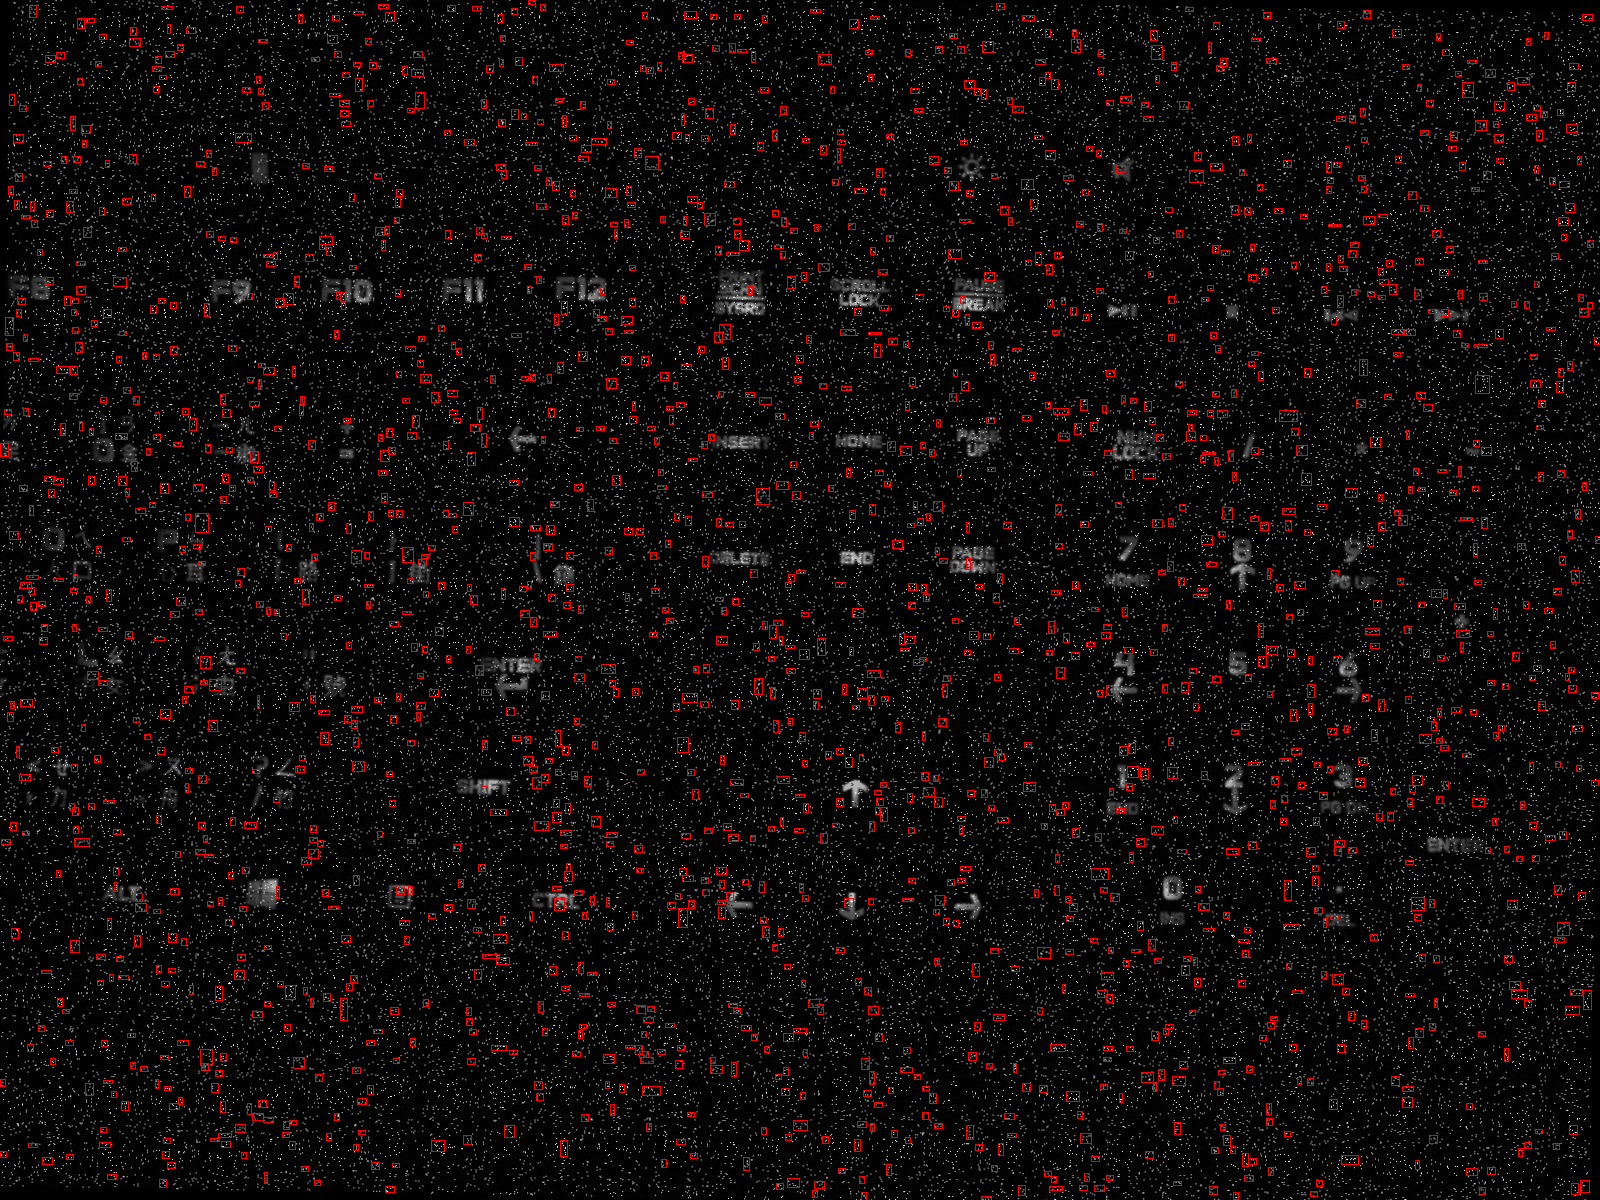
\includegraphics[width=0.5\linewidth]{simulation/Rotation/20/surf_showDefect.png}
			}
			\caption{Example of Bad Alignment Images, Here Shows the Absolute Difference Result after Defect Detection.}
			\label{fig:rotatinoBadAlignmentResult}
		\end{figure}

	\subsection{Unexpected Translation}
		In this section, we'll move the sample image \ref{fig:testSamplesOfTranslation} from left to right by 30, 50, 100, 200 pixels then observe the difference between each feature detector. 
		In this case, every feature point detector except ORB could have good result if the sample image contains every key caps letterings. In the case of unexpected translation. The behavior of ORB was too unstable, and this is not suitable for our application.
		ORB feature detector doesn't have very good performance when the sample image have almost any unexpected translation
		In the experiment, we didn't consider the overstated case since the fixture actually wouldn't allowing such amount of translation from happening. 
		A two centimeter translation would cause only about 100 pixels of translation in our camera viewing setup.
		\begin{figure}[H]
			\subfigure[Reference Image]
			{
				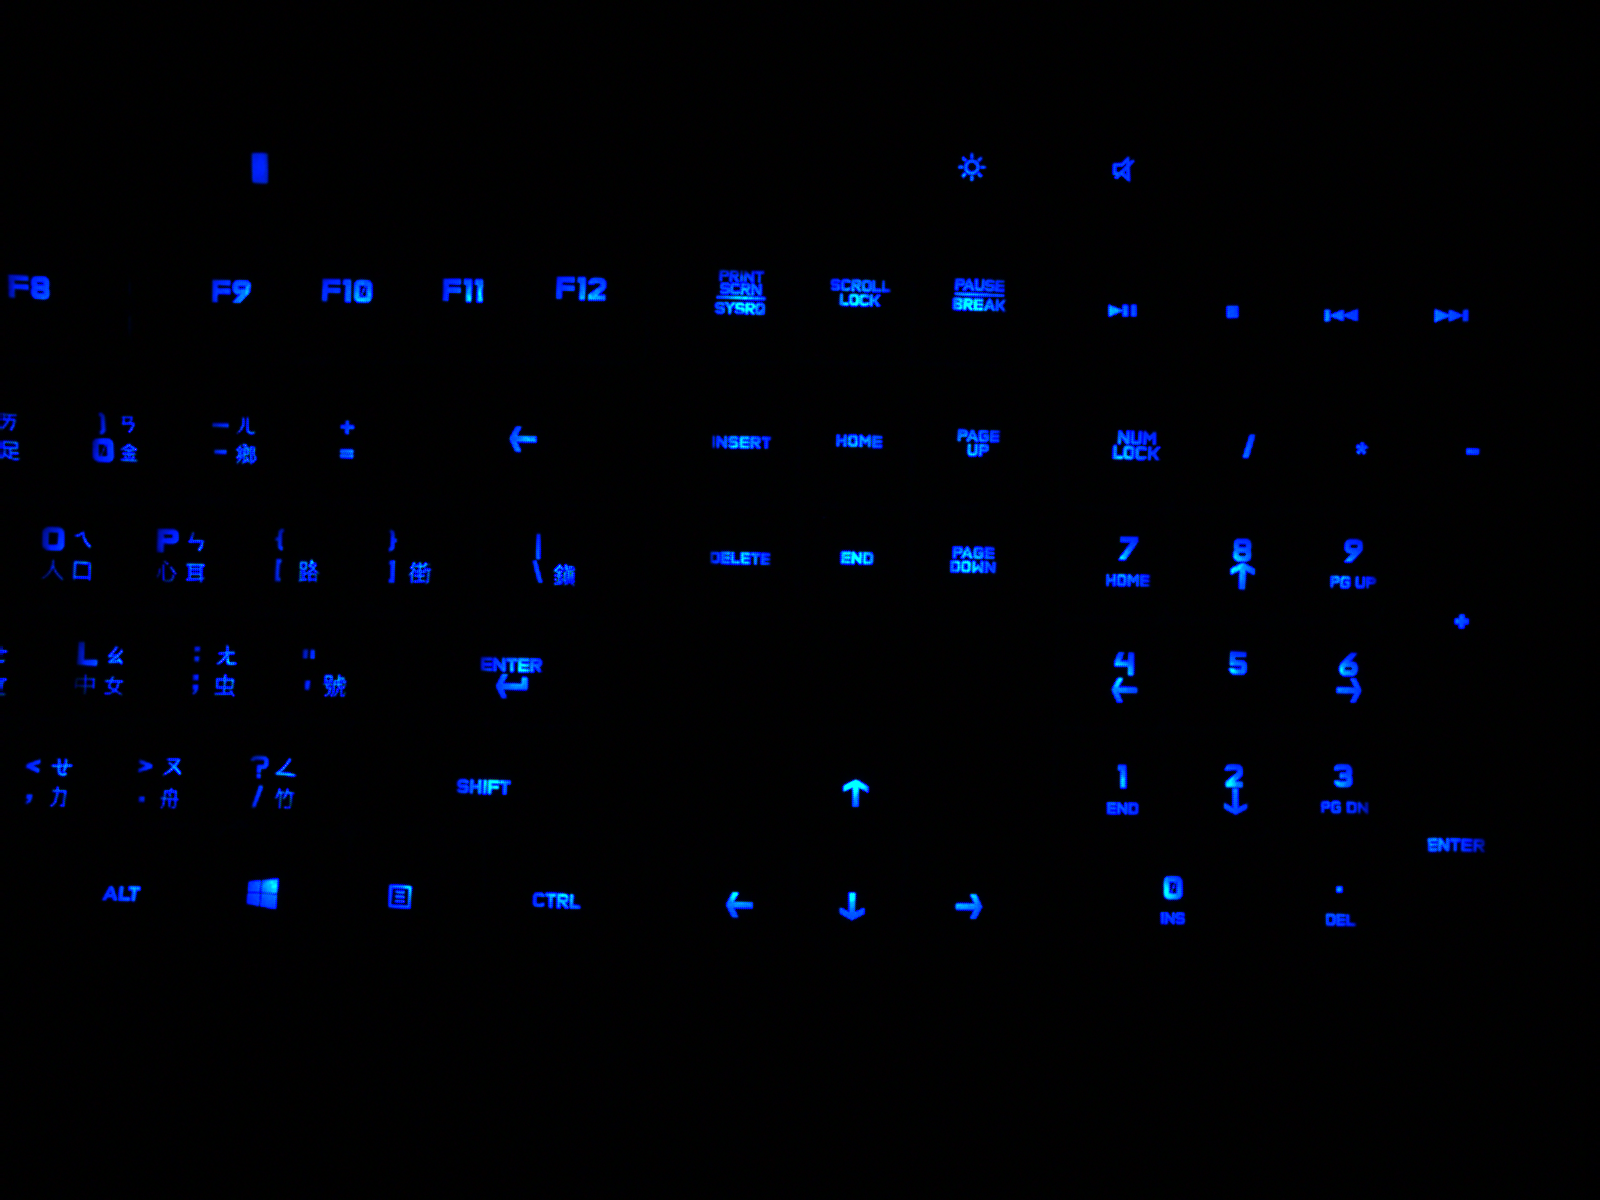
\includegraphics[width=\linewidth]{simulation/normal/input_gold.png}
			}
			\subfigure[Sample Image with 30 Pixels Translation]
			{
				\includegraphics[width=0.5\linewidth]{simulation/Translation/30/input_sample.png}
			}
			\subfigure[Sample Image with 50 Pixels Translation]
			{
				\includegraphics[width=0.5\linewidth]{simulation/Translation/50/input_sample.png}
			}
			\subfigure[Sample Image with 100 Pixels Translation]
			{
				\includegraphics[width=0.5\linewidth]{simulation/Translation/100/input_sample.png}
			}
			\subfigure[Sample Image with 200 Pixels Translation]
			{
				\includegraphics[width=0.5\linewidth]{simulation/Translation/200/input_sample.png}
			}
			\caption{Rotated Sample Image}
			\label{fig:testSamplesOfTranslation}
		\end{figure}

		\begin{figure}[H]
			\subfigure[ORB Feature Detectors Result in 30 Pixels Translation]
			{
				\includegraphics[width=0.5\linewidth]{simulation/Translation/30/orb_showDefect.png}
			}
			\subfigure[ORB Feature Detectors Result in 50 Pixels Translation]
			{
				\includegraphics[width=0.5\linewidth]{simulation/Translation/50/orb_showDefect.png}
			}
			\subfigure[ORB Feature Detectors Result in 100 Pixels Translation]
			{
				\includegraphics[width=0.5\linewidth]{simulation/Translation/100/orb_showDefect.png}
			}
			\subfigure[ORB Feature Detectors Result in 200 Pixels Translation]
			{
				\includegraphics[width=0.5\linewidth]{simulation/Translation/200/orb_showDefect.png}
			}
			\caption{Example of Bad Alignment Images, Here Shows the Absolute Difference Result after Defect Detection.}
			\label{fig:translationBadAlignmentResult}
		\end{figure}

	\subsection{LED failure}
		In this section, we'll mask out the sample image by deferent percentages then observe the difference between each feature detector.
		The following images \ref{fig:testSamplesOfMaskOut} were results by mask out the sample image by 20\%, 40\%, 60\%, 80\%, 85\%, 90\% and 95\%.
		In this case, both SIFT ans SURF could have good alignment result when the masked area lower then 90\%, witch have the best performance.
		AKAZE obtains good alignment up to 60\% of sample image were masked, start to have bad alignment when 80\% of sample image were masked.
		For ORB, thought having the best time efficiency, ORB is the most unreliable feature detector in this case, have bad alignment result when the masked area is larger then 40\%.
		\begin{figure}[H]
			\subfigure[Reference Image]
			{
				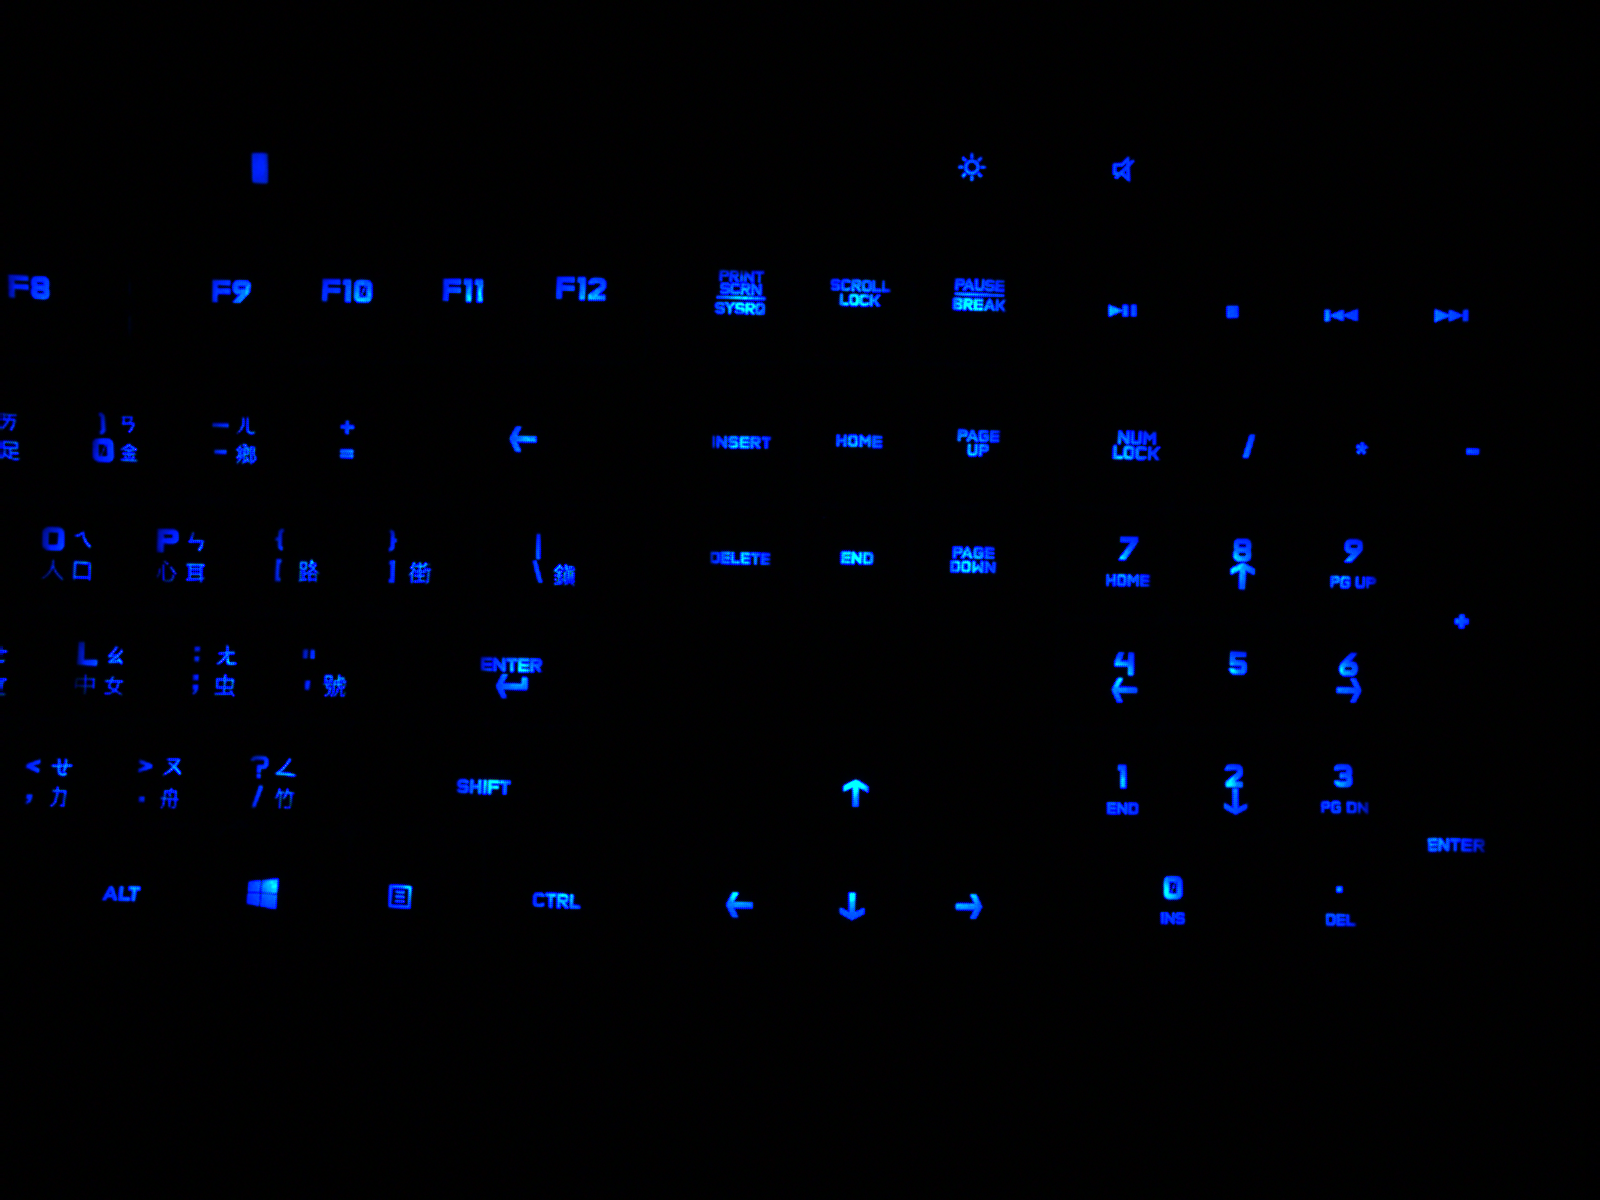
\includegraphics[width=0.3\linewidth]{simulation/normal/input_gold.png}
			}
			\subfigure[Sample Image with 20\% Masked Area]
			{
				\includegraphics[width=0.3\linewidth]{simulation/Masking/20/input_sample.png}
			}
			\subfigure[Sample Image with 40\% Masked Area]
			{
				\includegraphics[width=0.3\linewidth]{simulation/Masking/40/input_sample.png}
			}
			\subfigure[Sample Image with 60\% Masked Area]
			{
				\includegraphics[width=0.3\linewidth]{simulation/Masking/60/input_sample.png}
			}
			\subfigure[Sample Image with 80\% Masked Area]
			{
				\includegraphics[width=0.3\linewidth]{simulation/Masking/80/input_sample.png}
			}
			\subfigure[Sample Image with 85\% Masked Area]
			{
				\includegraphics[width=0.3\linewidth]{simulation/Masking/85/input_sample.png}
			}
			\subfigure[Sample Image with 90\% Masked Area]
			{
				\includegraphics[width=0.3\linewidth]{simulation/Masking/90/input_sample.png}
			}
			\subfigure[Sample Image with 95\% Masked Area]
			{
				\includegraphics[width=0.3\linewidth]{simulation/Masking/95/input_sample.png}
			}
			\caption{Sample Image Simulating The LED Failure}
			\label{fig:testSamplesOfMaskOut}
		\end{figure}
		\begin{figure}[H]
			\subfigure[SIFT Feature Detectors Result in 90\% Masked]
			{
				\includegraphics[width=0.5\linewidth]{simulation/Masking/90/sift_showDefect.png}
			}
			\subfigure[SURF Feature Detectors Result in 80\% Masked]
			{
				\includegraphics[width=0.5\linewidth]{simulation/Masking/80/SURF_showDefect.png}
			}
			\subfigure[ORB Feature Detectors Result in 80\% Masked]
			{
				\includegraphics[width=0.5\linewidth]{simulation/Masking/80/akaze_showDefect.png}
			}
			\subfigure[ORB Feature Detectors Result in 40\% Masked]
			{
				\includegraphics[width=0.5\linewidth]{simulation/Masking/40/orb_showDefect.png}
			}
			\caption{Example of Bad Alignment Images, Here Shows the Absolute Difference Result after Defect Detection.}
			\label{fig:masekdBadAlignmentResult}
		\end{figure}
	\subsection{Noise of Camera}
		In this section, we'll add the salt \& pepper noise with different level to the sample image, then observe the difference between each feature detector.

\section{Comparison between each Feature Detector}
	% add execiution time compare chart here
	\subsection{Simple Blob Detector}
		\subsubsection{Introduction}
			The blob feature detector is an simple approach for feature point detection. We choose the centroid of each selected blob as the feature point. Matching feature points with nearest neighborhood. 
			Since we have a fixture that can guarantee the keyboard does not have shift or rotation more then a certain amount, we can assume that the feature point matched is the nearest one.
		\subsubsection{Performance}
			% $$\textrm{Add time data}$$
		\subsubsection{Pros \& Cons}
			This method has lowest robustness in experiment, but fastest in execution.

	\subsection{SIFT}
		\subsubsection{Introduction}
		SIFT feature is proposed by Lowe \cite{lowe2004distinctive} et al., having the state of the art robustness in most scenarios \cite{karami2017image}, but slower than any other methods on execution.
		\subsubsection{Performance}
			% $$\textrm{Add time data}$$
		\subsubsection{Pros \& Cons}
	
	\subsection{SURF}
		\subsubsection{Introduction}
		SURF is a upgrade version based on SIFT, witch is designed to solve the speed issue of SIFT. 
		And in the scenario of this thesis, this method meets the requirement on the stability without wasting too much time on calculation.
		\subsubsection{Performance}
			% $$\textrm{Add time data}$$
		\subsubsection{Pros \& Cons}

	\subsection{ORB}
		\subsubsection{Introduction}
		ORB is a
		\subsubsection{Performance}
			% $$\textrm{Add time data}$$
		\subsubsection{Pros \& Cons}

	\subsection{AKAZE}
		\subsubsection{Introduction}
		AKAZE is a
		\subsubsection{Performance}
			% $$\textrm{Add time data}$$
		\subsubsection{Pros \& Cons}